\chapter{Self-Balancing Robot}\label{sec: BalancingRobot}
In this chapter, the objective is to address the inverted pendulum problem through the usage of an FPGA in coexistence with a microcontroller. For this, in the respective chapters, physics of a self-balancing robot, the calculation of its structure, the sensors and actuators used, the control system and the design and manufacture of a PCB that solves in a more adequate way some problems of those previously raised, will be treated.A communication between FPGA/Microcontroller will be used and a more global version of the proposed system will be given, with a general block diagram. \newline

It starts with a problem description (section \ref{sec:Descripcion_balancin}) to continue with a brief high level solution (section \ref{sec:Diseno}). To finish, an explanation of each blocks will be described (section \ref{sec:Implementacion}).

\section{Problem Description} \label{sec:Descripcion_balancin}

To understand the work to be done, the problem of inverted pendulum will be briefly enunciated, whose solution has given rise to many very famous tools nowadays, one of them, called \textit{SegWay} (Figure \ref{fig:segway}).

\begin{figure}[H]
	\center
	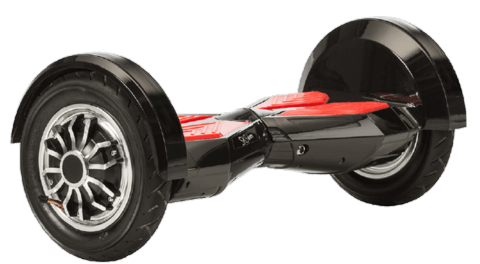
\includegraphics[trim = 0mm 0mm 0mm 0mm, clip,scale=0.4]{imagenes/Balancing_robot/segway}
	\caption{Commercial Segway.}
	\label{fig:segway}
\end{figure}


\begin{definicion}Pendulum \cite{Pendulum}: It is a physical system that can oscillate under the gravitational action or other physical characteristic (elasticity, for example) and that is configured by a mass suspended from a point or a horizontal axis by a wire, a rod, or other device that is used to measure time. \newline
\end{definicion}
As can be imagined, an inverted pendulum has the aspect shown in Figure \ref{fig:pendulo}. 

\begin{figure}[H]
	\center
	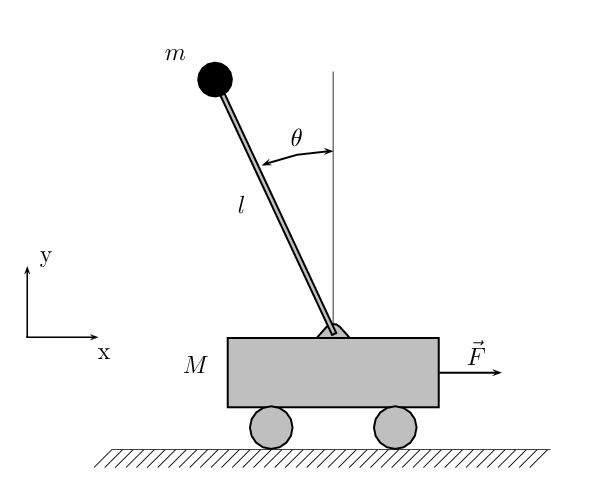
\includegraphics[trim = 0mm 0mm 0mm 0mm, clip,scale=1.6]{imagenes/Balancing_robot/pendulo}
	\caption{Inverted pendulum representation.}
	\label{fig:pendulo}
\end{figure}

Consists of a pendulum where the mass center is located above the point or balancing axis. As expected, this layout gives the system static instability. We recall that a system is stable when its gravity center is closer to the support horizontal plane. \newline

The base of this project will therefore be to correct this instability and is part of one of the most famous problems in terms of control theory and systems dynamics. 

\newpage
\section{System Design}\label{sec:Diseno}

By i2c communication with an IMU sensor, the microcontroller obtains the current angle of the system. Obtained the angle by the microcontroller a communication of serial type sends it to the FPGA in a binary format of 1 byte for the integral part and 1 byte for the decimal part. A shield with a driver of DC motors connected to the FPGA brings the possibility of varying the speed and direction of two DC motors that allow the stabilization of the system. The speed of the motors for a correct correction of the angle is calculated by a basic PD controller implemented in the FPGA.

\begin{center}
	\begin{figure}[H]
		\center
		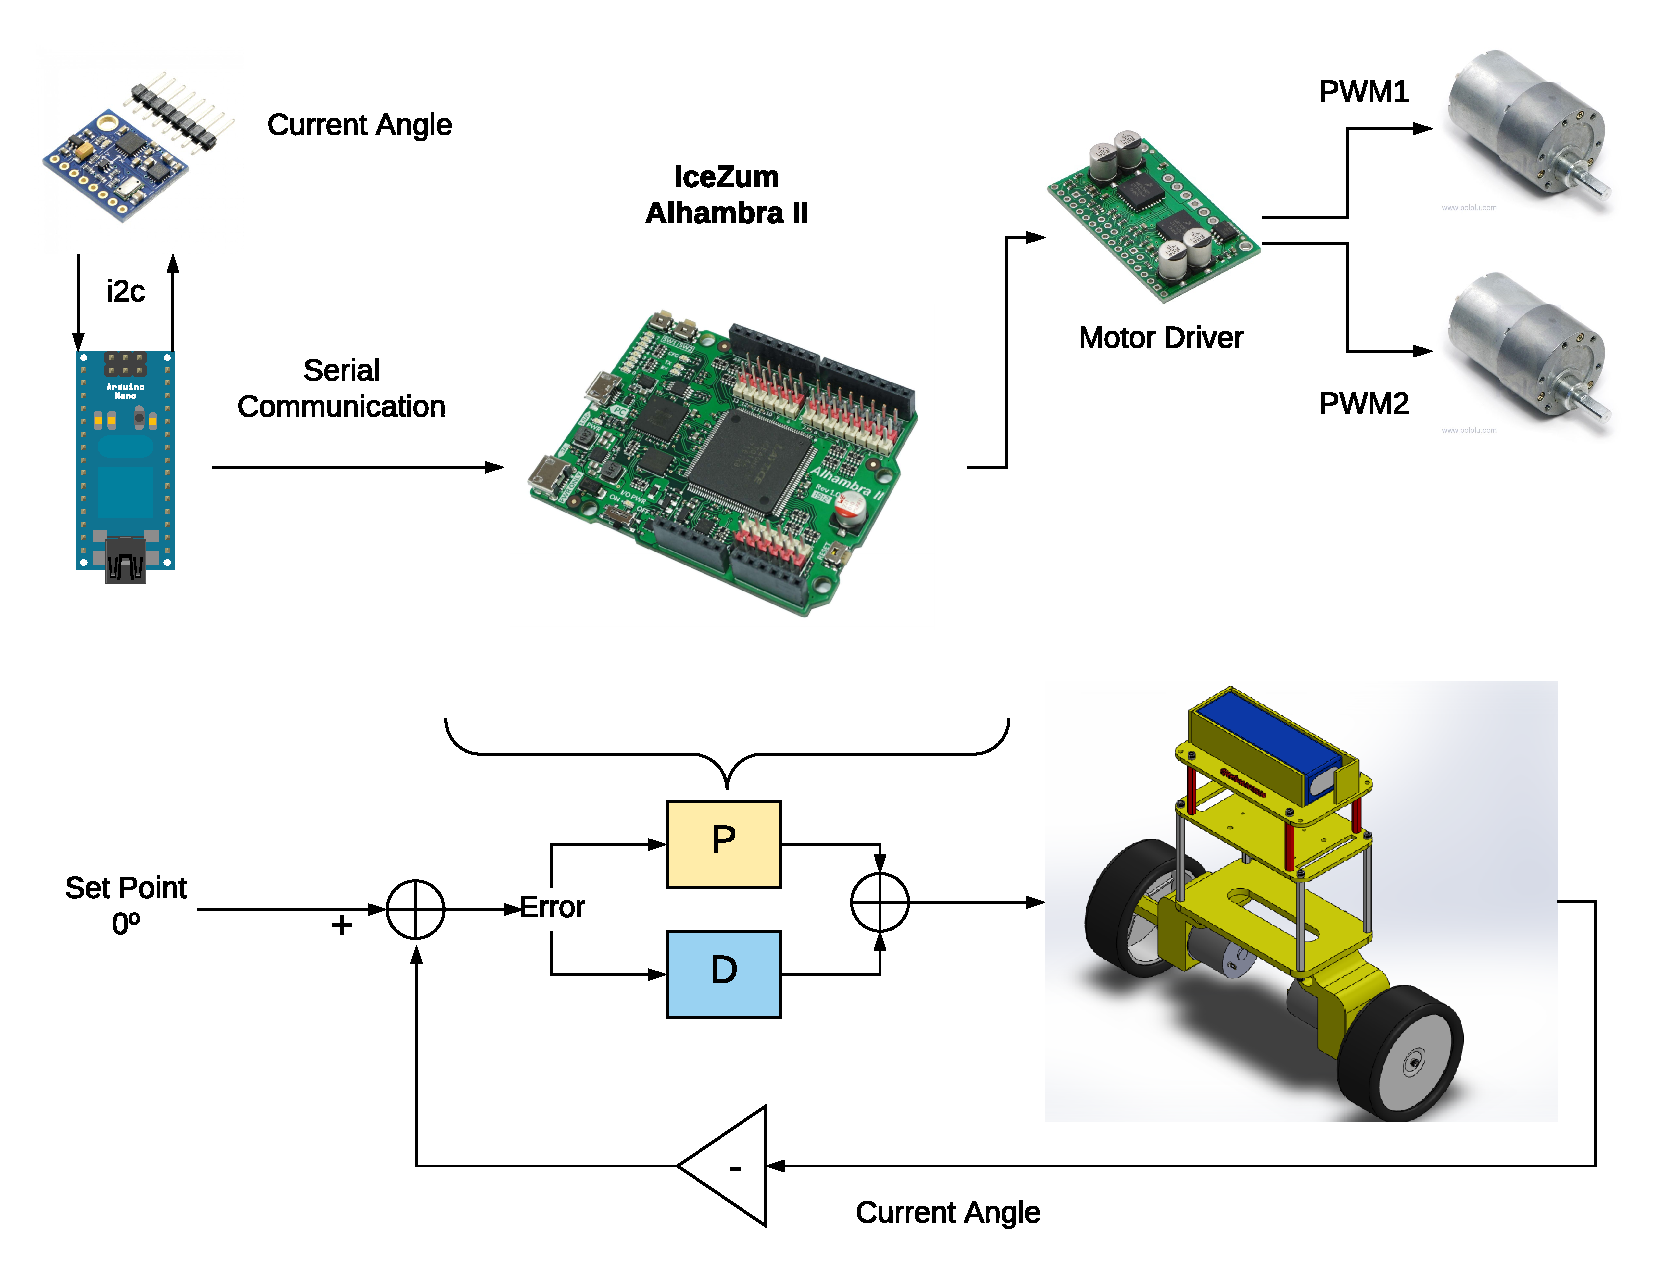
\includegraphics[trim = 0mm 0mm 0mm 0mm,clip, angle=0, scale = 0.4]{imagenes/Balancing_Robot/final.pdf}
		\caption{Final block diagram.}
		\label{fig:final}
	\end{figure}
\end{center}

%En esta sección se propone una solución al problema planteado proporcionando esta con un alto nivel de abstracción. En la sección \ref{sec:Implementacion} se profundizará aún más en los detalles de los diferentes sub-sistemas que aquí se exponen.

The following chapters will go deeper into each of the previous blocks that form the final solution (Figure \ref{fig:final}). 


\newpage
\section{System Implementation}\label{sec:Implementacion}
\subsection{Mechanical Structure Manufacturing}
Knowing the physics of a self-balancing robot \cite{6845943} \cite{7112017} and with the aim, therefore, of solving the classic problem of the inverted pendulum, the mechanical structure of the Figures \ref{fig:EnsanBalanceFront}, \ref{fig:EnsanBalanceLateral} y \ref{fig:EnsanBalanceCab},designed with SolidWorks[] is proposed and from which the rest of the components will be assembled.

\begin{center}
	\begin{figure}[H]
		\center
		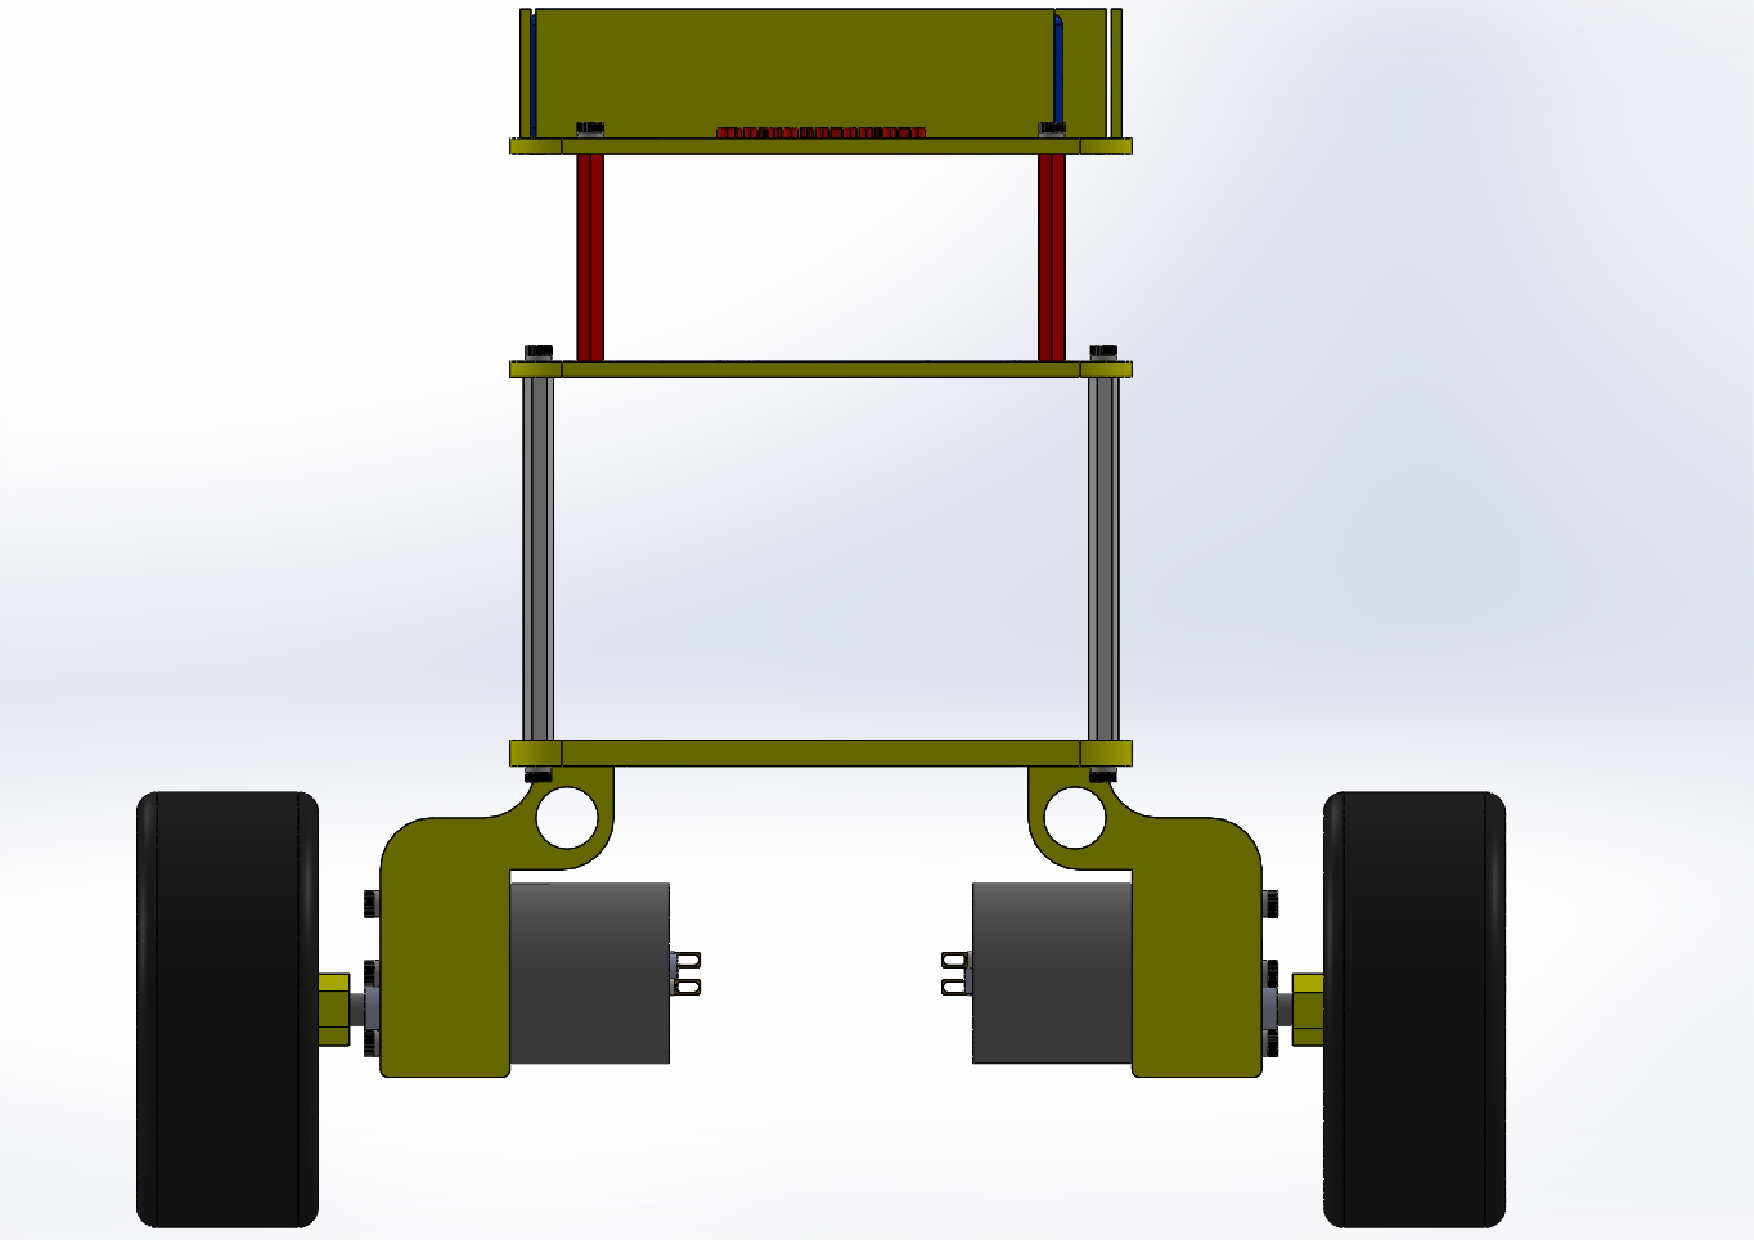
\includegraphics[trim = 1cm 0mm 2.7cm 0mm,clip, angle=0, scale = 0.4]{imagenes/Balancing_Robot/EnsanBalanceFront.PDF}
		\caption{Frontal view Balancing Robot.}
		\label{fig:EnsanBalanceFront}
	\end{figure}
\end{center}

\begin{center}
	\begin{figure}[H]
		\center
		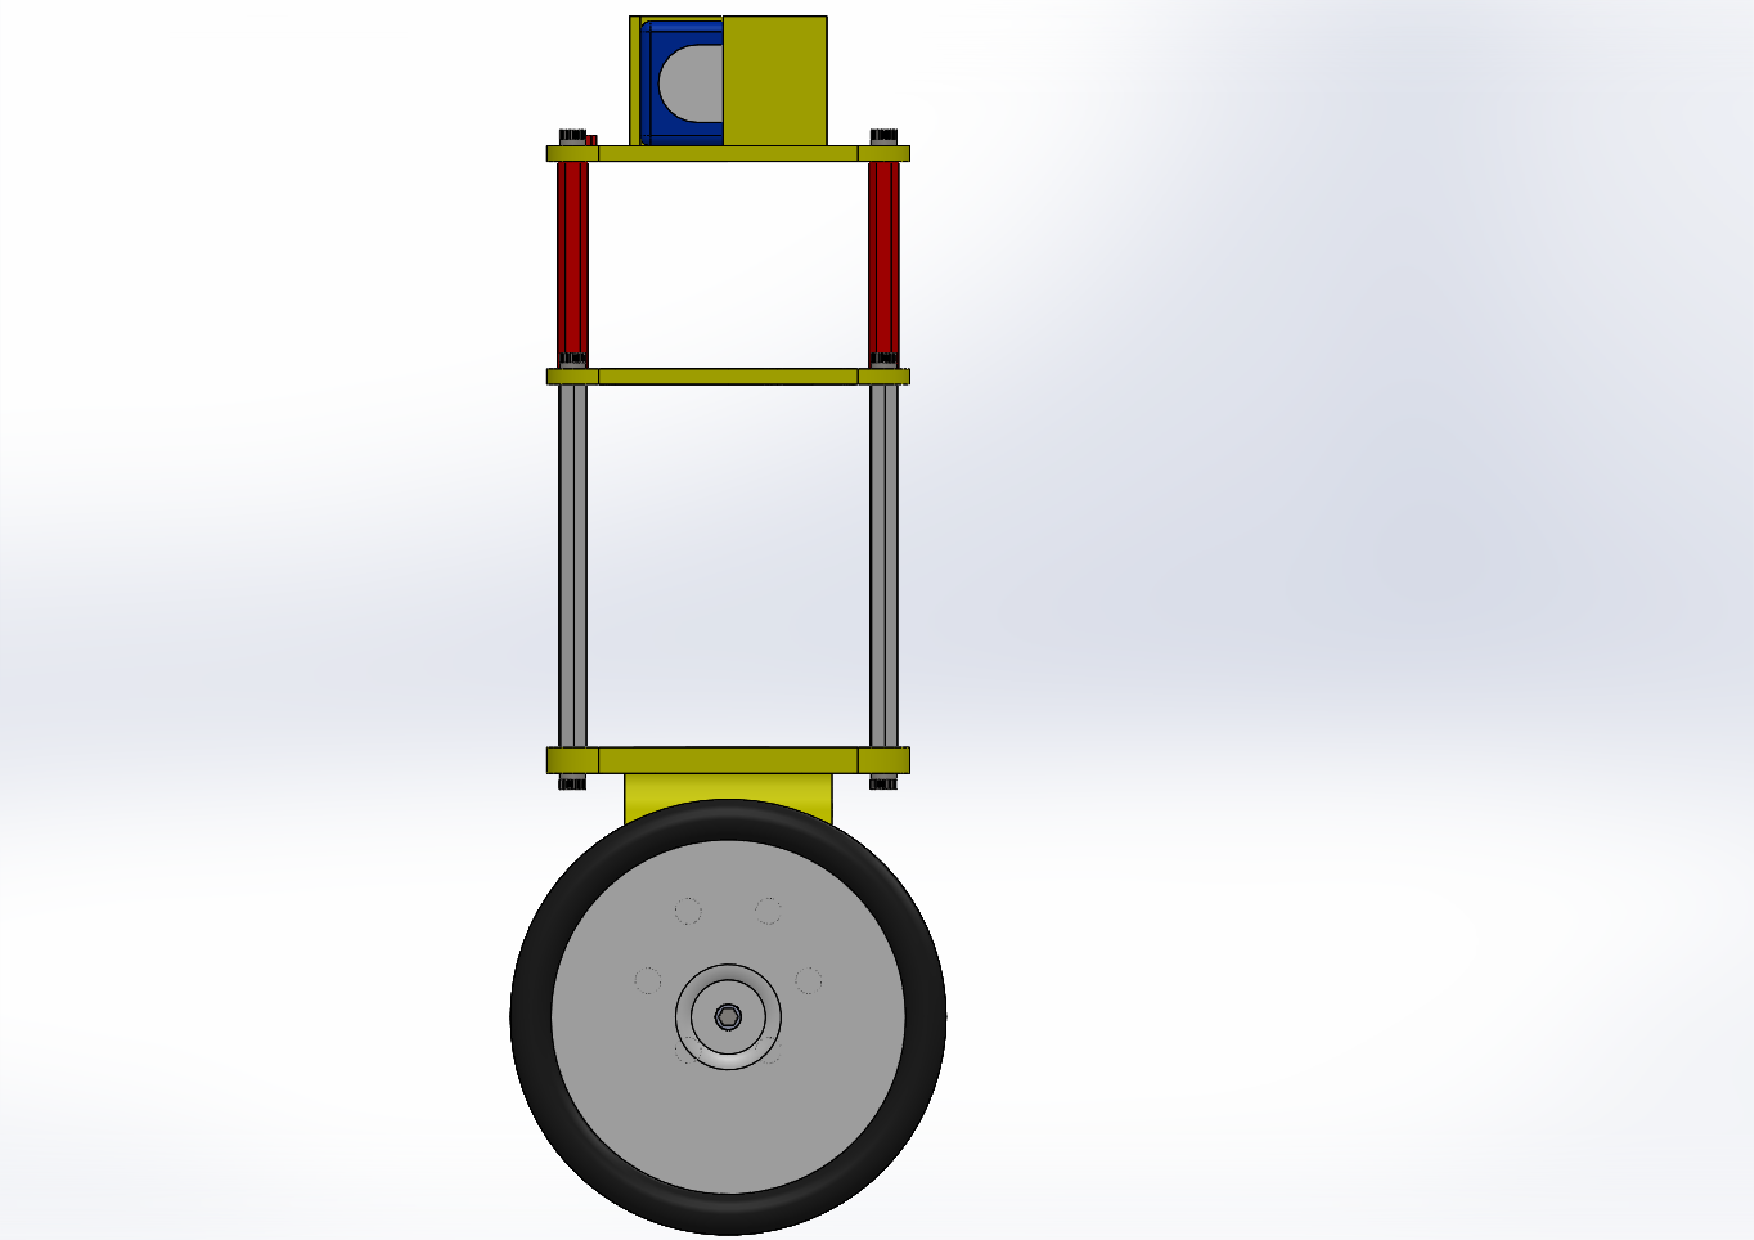
\includegraphics[trim = 5cm 0mm 10cm 0mm,clip, angle=0, scale = 0.5]{imagenes/Balancing_Robot/EnsanBalanceLateral.PDF}
		\caption{Lateral view derecha Balancing Robot.}
		\label{fig:EnsanBalanceLateral}
	\end{figure}
\end{center}

\begin{center}
	\begin{figure}[H]
		\center
		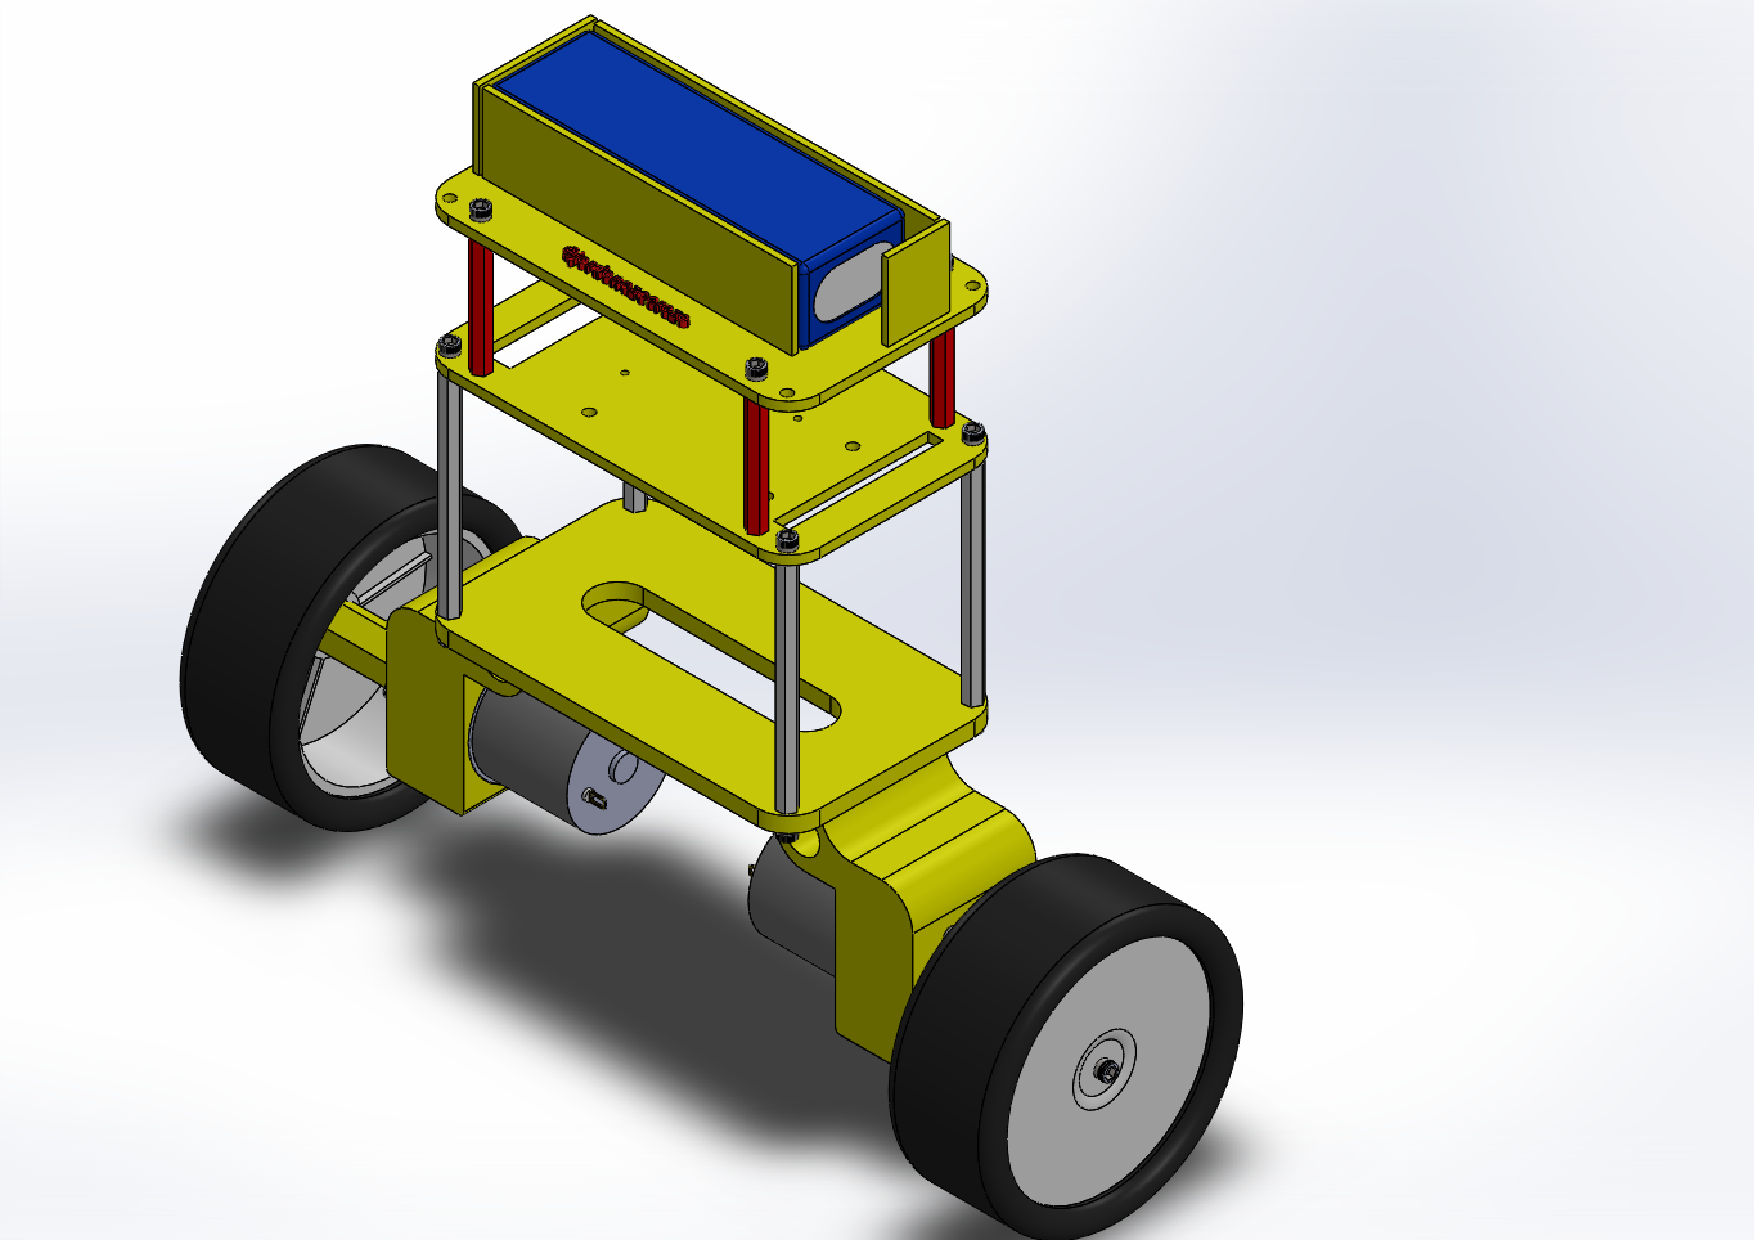
\includegraphics[trim = 20mm 0mm 8cm 0mm,clip, angle=0, scale = 0.5]{imagenes/Balancing_Robot/EnsanBalanceCab.PDF}
		\caption{Balancing Robot perspective.}
		\label{fig:EnsanBalanceCab}
	\end{figure}
\end{center}

Different aspects of the design of this structure are considered, which are directly related to the physics of a self-balance Robot, and with it, of the inverted pendulum. \newline
As argued in section \ref{sec:Descripcion_balancin}, a system at rest is stable when its mass center is closer to the horizontal plane. If we consider that the nature of the proposed system is inherently unstable, it is necessary to know the best point where the mass center must be in order to allow a better stability. \newline

Assuming the of mathematical modeling characterization[][], it is therefore assumed that to achieve greater ease in stabilization, the center of mass should be placed above the midpoint of the vertical axis of our system. Therefore, we must consider the weight of all components for a placement that allows the above. \newline
In Figure \ref{fig:center_mass}, a SolidWorks calculation is represented from this mass center where there have only been considered the heavier components of the final system, which includes, DC motors, batteries, mechanical structures and wheels.

\begin{figure}[H]
	\center
	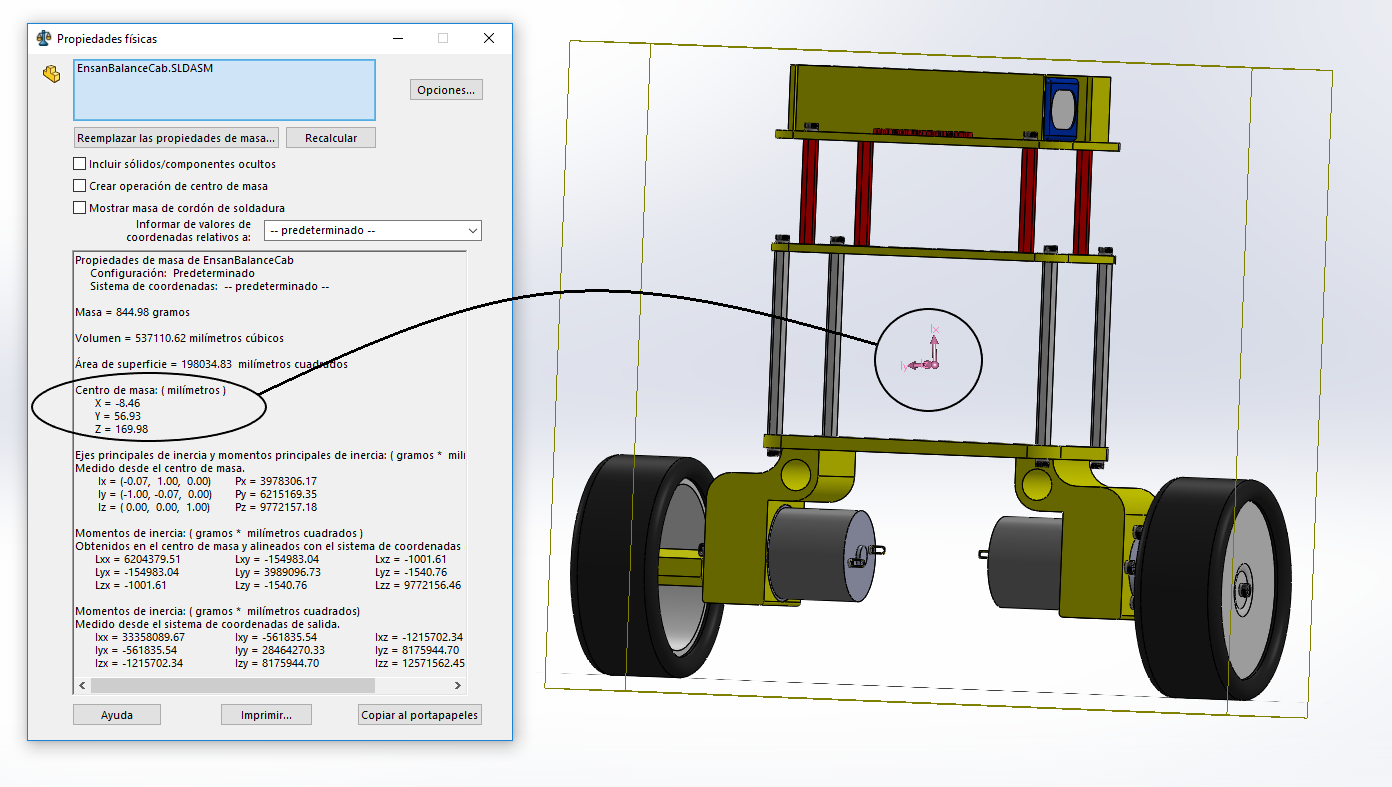
\includegraphics[scale=0.3]{imagenes/Balancing_robot/center_mass}
	\caption{Center of mass final system.}
	\label{fig:center_mass}
\end{figure}

\subsection{Inertial Measurement Unit MPU6050 in Arduino Nano}\label{sec:MPU6050}

A constant knowledge of the angle of the system is necessary for its analysis and correction, for this purpose the MPU6050 sensor has been used, connected by an i2c communication to an Arduino Nano. \newline

The MPU6050[] is an Inertial Measure Unit (IMU) with 6 degrees of freedom (6DOF) manufactured by Invensense[]. It has an accelerometer and gyroscope and allows communication by both SPI and i2c bus. To correct some of the data collection problems, mentioned in section \ref{sec:IMU} it incorporates an internal processor (Digital Motion Processor, DMP) that executes data fusion algorithms (Motion Fusion) to combine the measurements of the internal sensors, avoiding having to perform the filters externally.\newline

Due to its low cost and big quality, this is one of the most used IMUs nowadays. In Figure \ref{fig:IMU1} a MPU6050 image is shown.

\begin{figure}[H]
	\center
	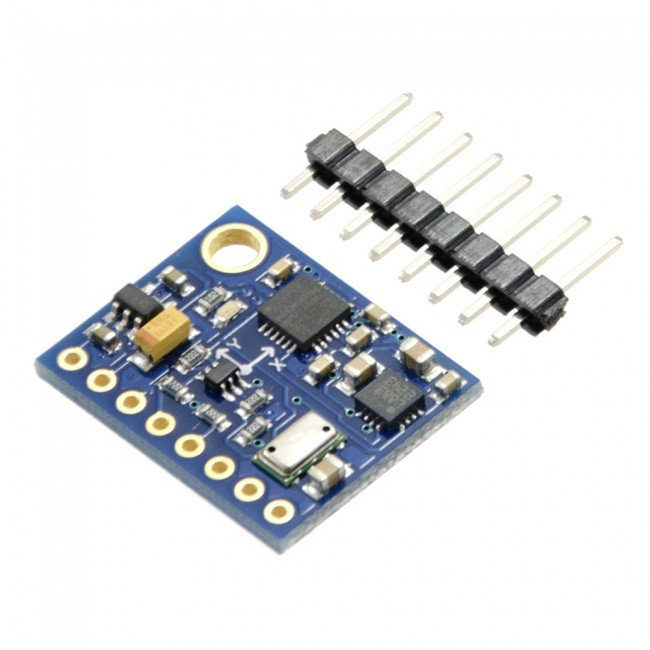
\includegraphics[scale=0.2]{imagenes/Balancing_robot/IMU1}
	\caption{MPU6050 IMU.}
	\label{fig:IMU1}
\end{figure}
\subsubsection{Pin-out}

Figure \ref{fig:MPU6050_schematic} shows the schematic connections diagram of the MPU6050.

\begin{figure}[H]
	\center
	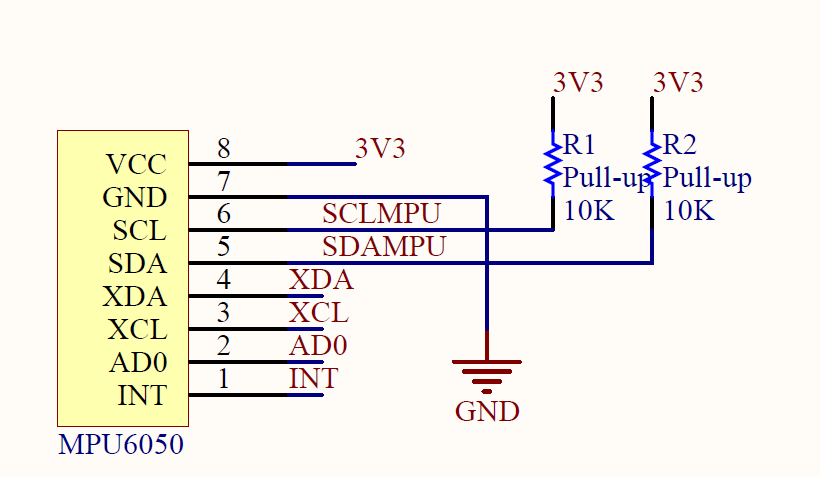
\includegraphics[scale=0.4]{imagenes/Balancing_robot/MPU6050_schematic}
	\caption{MPU6050 IMU.}
	\label{fig:MPU6050_schematic}
\end{figure}

It has a 3.3V power supply voltage. The clock pin for the I2C connection (Serial Clock Line, SCL) and the data pin (Serial Data Line, SDA) represent the connection for the bus with Arduino Nano. AD0 pin allows the user to change the address of the MPU (slave), which by default is 0x68h connected to GND. If it is connected to Vcc, the address changes to 0x69h. INT pin produces a signal on high when the data in issue is available from the MPU to be captured and will warn by an interruption to the Arduino Nano with the purpose to be obtained.\newline

\subsubsection{Arduino Nano Program}
For the Arduino Nano implementation it is used a library developed by Jeff Rowberg[]. The reason of the use of this library is because it incorporates the usage of the DMP. This use  exempts the microprocessor (Arduino Nano in this case) from a complex filtered and calculation with the purpose to obtain the values pitch, yaw and roll. A representation of this advantages are represented in Figure \ref{fig:DMPExample}.\newline
\begin{figure}[H]
	\center
	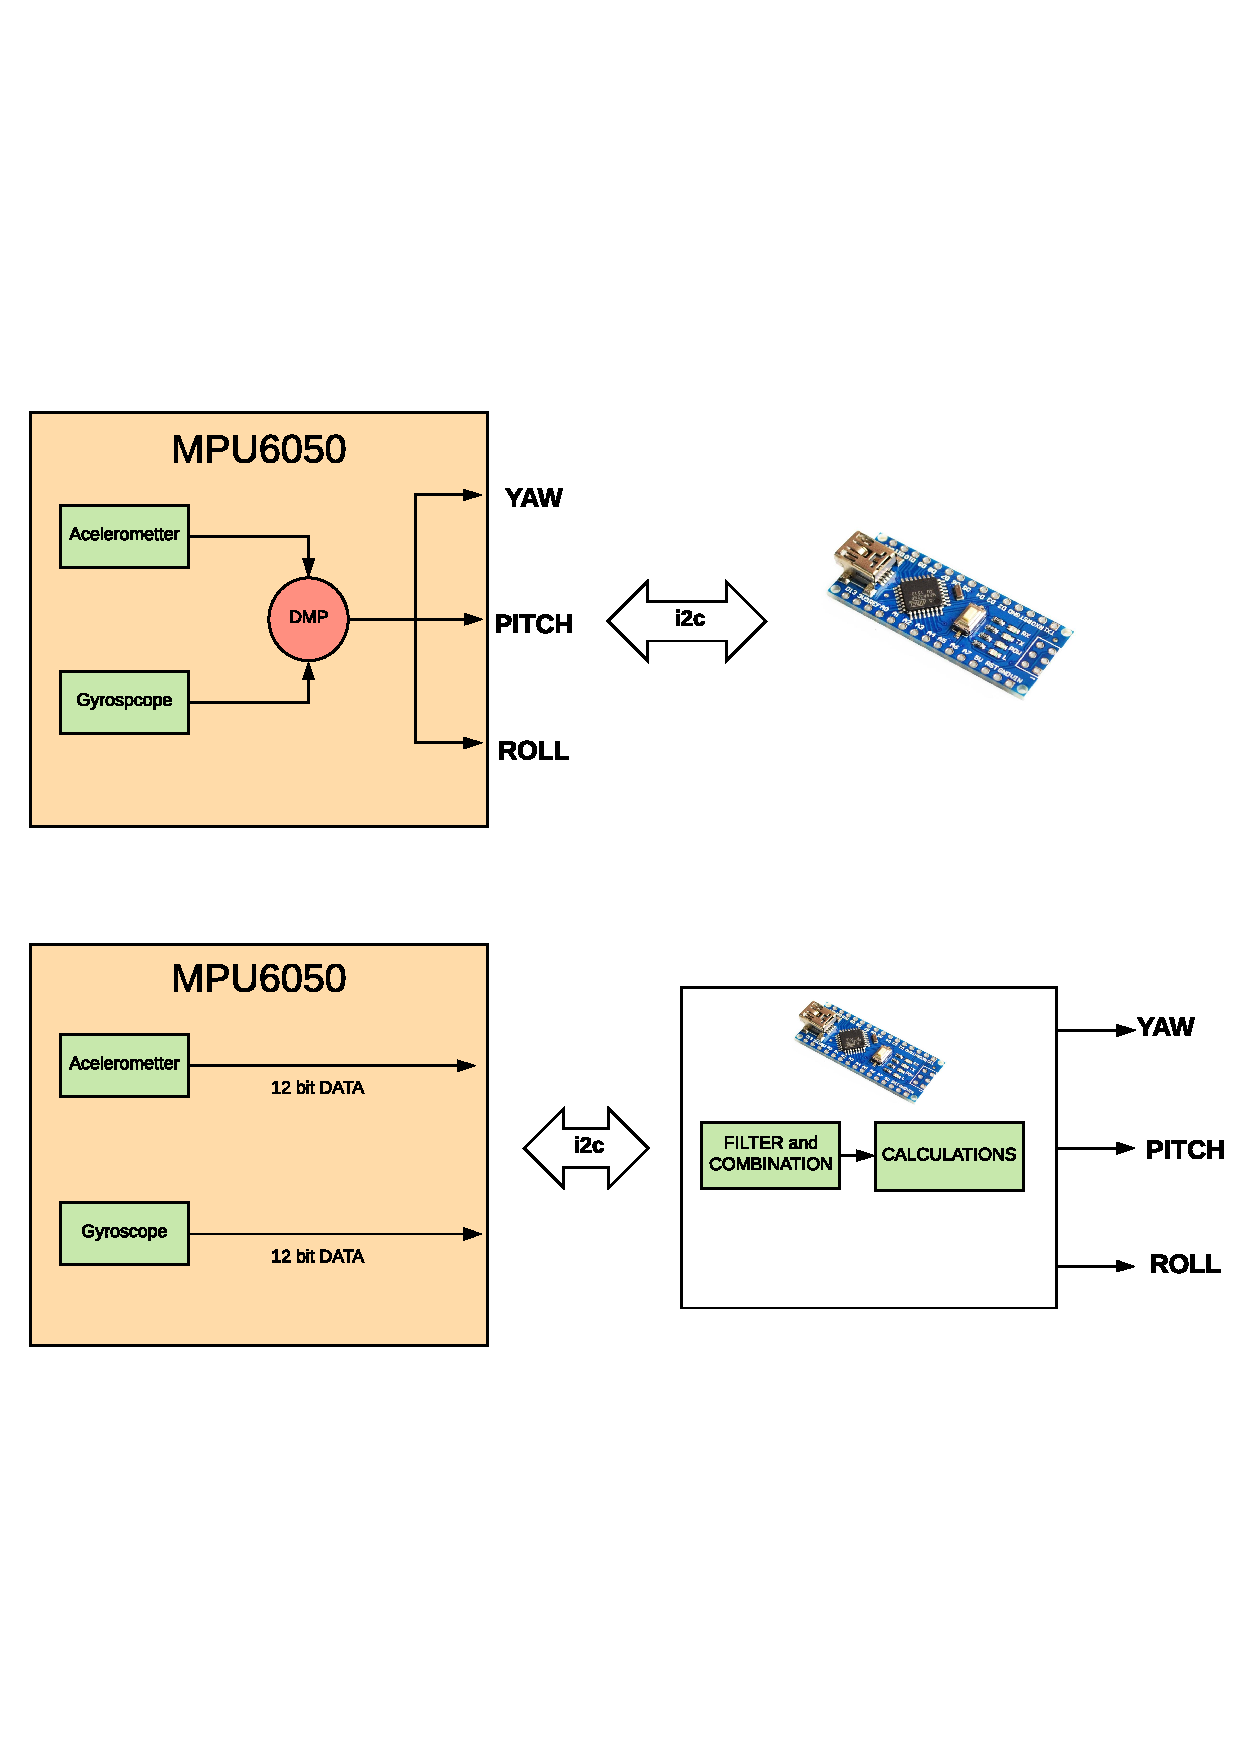
\includegraphics[trim = 0mm 4cm 0mm 2cm, clip,scale=0.6]{imagenes/Balancing_robot/DMPexample.pdf}
	\caption{Advantaje in the use of DMP.}
	\label{fig:DMPExample}
\end{figure} 


%An example of the obtained values by the sensor are shown in the figure.

%\textbf{foto de un ejemplo de los ángulos}

\subsection{Implementación PCB}\label{sec:PCB}

After featuring the entire system and considering the necessary connection diagram not only between the microcontroller and FPGA but also for the OV7670 (it uses in section \ref{sec: Cuadricoptero}) and the motor driver, it is convenient and appropriate a printed circuit that solves some noise problems, excessive cables, etc. \newline

The printed circuit contains the following components and behaviors:

\begin{itemize}
	\item A total of 28 pins on the outside of the PCB and arranged in the correct position for a fit in the IceZum Alhambra II board (Figure \ref{fig:pin_headers}), which allows to use as inputs or outputs the pins of the FPGA. In order to know the exact position of the pins on the plate, the Altium project was used, which is available on GitHub.
	
	\begin{figure}[H]
		\center
		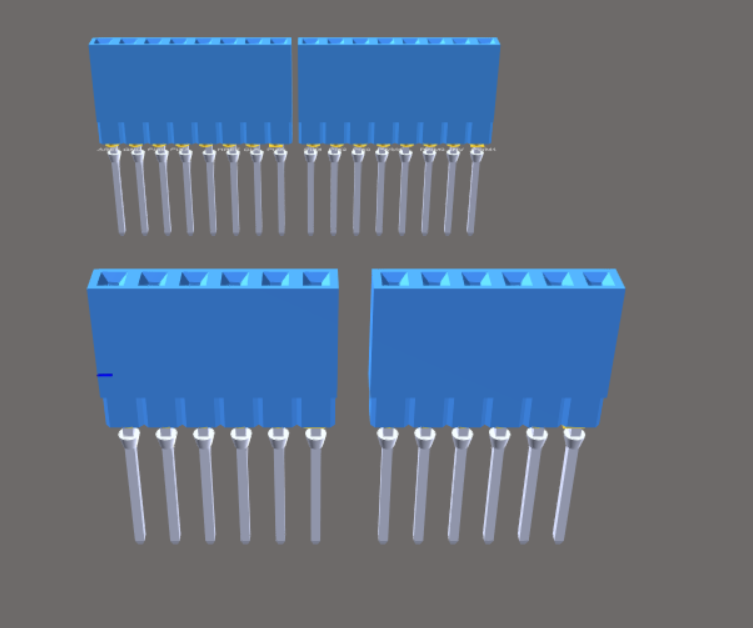
\includegraphics[scale=0.4]{imagenes/Balancing_robot/pin_headers.PNG}
		\caption{Pin headers for IceZum Alhambra II.}
		\label{fig:pin_headers}
	\end{figure}
	
	
	\item 4 VDC and 12 Volt GND connections to power the ESCs of the brushless motors of the aerial vehicle. For this, the component of figure \ref{fig:screw}, has been chosen, because it has adequate features of maximum temperature to which it may be subjected and which would be analyzed further on.
	
	\begin{figure}[H]
		\center
		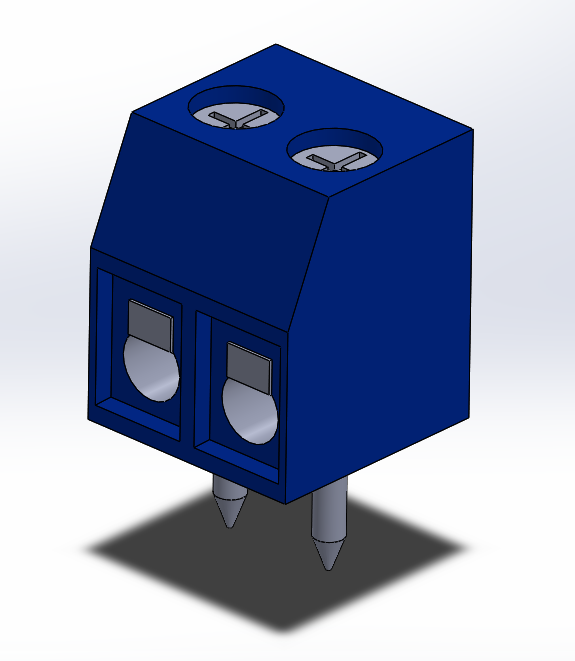
\includegraphics[scale=0.4]{imagenes/Balancing_robot/SCREW.PNG}
		\caption{Connector GND and VCC.}
		\label{fig:screw}
	\end{figure}
	
	
	\item A VCC and GND connection to feed the previous connections. This connector would go directly to a LIPO battery of 11.1V (3 cells) and 2200mAh. The fact of choosing this battery is due to the minimum voltage by which the ESCs of the brushless motors are fed, as well like the motors and the motor driver used for the self-balancing Robot. A more detailed analysis of the battery can be found in subsection \ref{sec:Bateria}
	
	\item Header pin modules for the MPU6050 connection previously described. (Figure \ref{fig:mpu6050_connector}).
		
		\begin{figure}[H]
			\center
			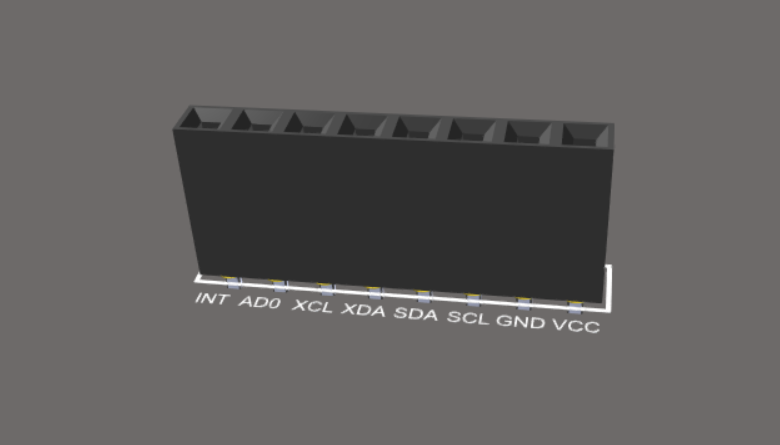
\includegraphics[scale=0.4]{imagenes/Balancing_robot/mpu6050_connector.PNG}
			\caption{Module MPU6050.}
			\label{fig:mpu6050_connector}
		\end{figure}
		
		\item An extension of the most important pins of the MPU6050 is made so that they can be used by the microcontroller in the case of angle analysis, as in this project, is part of a process governed by the microcontroller.
		
		\item Two jumpers connection (Figure \ref{fig:jumpers}) in I2C bus allow the user to decide who governs the SDA and SCL line, microcontroller or FPGA. 
		
		\begin{figure}[H]
			\center
			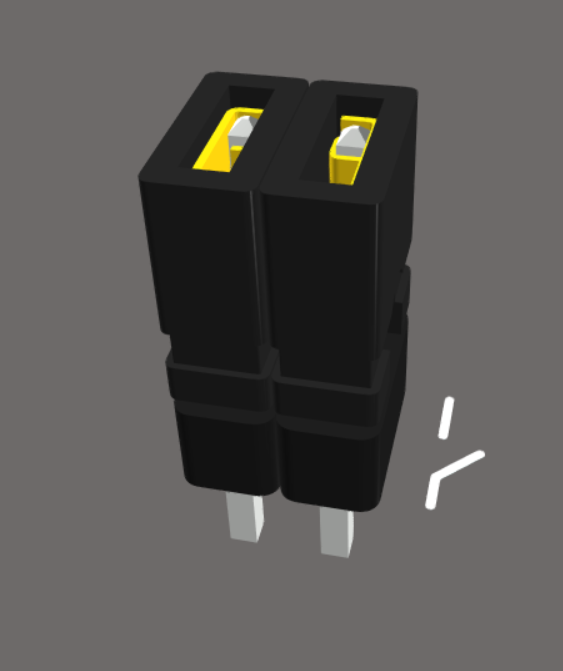
\includegraphics[scale=0.3]{imagenes/Balancing_robot/jumpers.PNG}
			\caption{Jumpers to configurate i2c MPU6050.}
			\label{fig:jumpers}
		\end{figure}	
	
		When hosting a bus line, it is not necessary to consider the thermal characteristics of the connector in issue, and when working at a relatively small frequency, the noise that the jumpers can introduce into the I2C communication may be accepted.
		\item A great part of actual microcontrollers works at 3.3-5V but the input voltage supported can go high to 12V, because of that it is taken advantage of the LIPO battery power and a new connector with two header pin is implemented that goes to VCC and GND which will power the microcontroller.	
		\item A module that can host the OV7670 camera (section \ref{sec: Cuadricoptero})formed by male headers pin and each of which will be attached to one of the FPGA's in-out pins, as will be seen later in the general schematic.
		\item A module that can host the driver of the DC motor used in this case and that allows direct connection with IceZum Alhambra II pins, for example, the pwm signal that will define the speed of the engines will be an output on one of the FPGA pins, and it should be an input to the motor driver.
		
		\item So that there are no errors in the I2C transmission, there’s a 4,7K$\Omega$ resistor in each of the lines.
	\end{itemize}	
	In Figures \ref{fig:top_3D}, \ref{fig:bottom_3D}, \ref{fig:Vista3D1}, \ref{fig:Vista3D2} is included a 3D representation of the final system with all its added component
	
	\begin{center}
		\begin{figure}[H]
			\center
			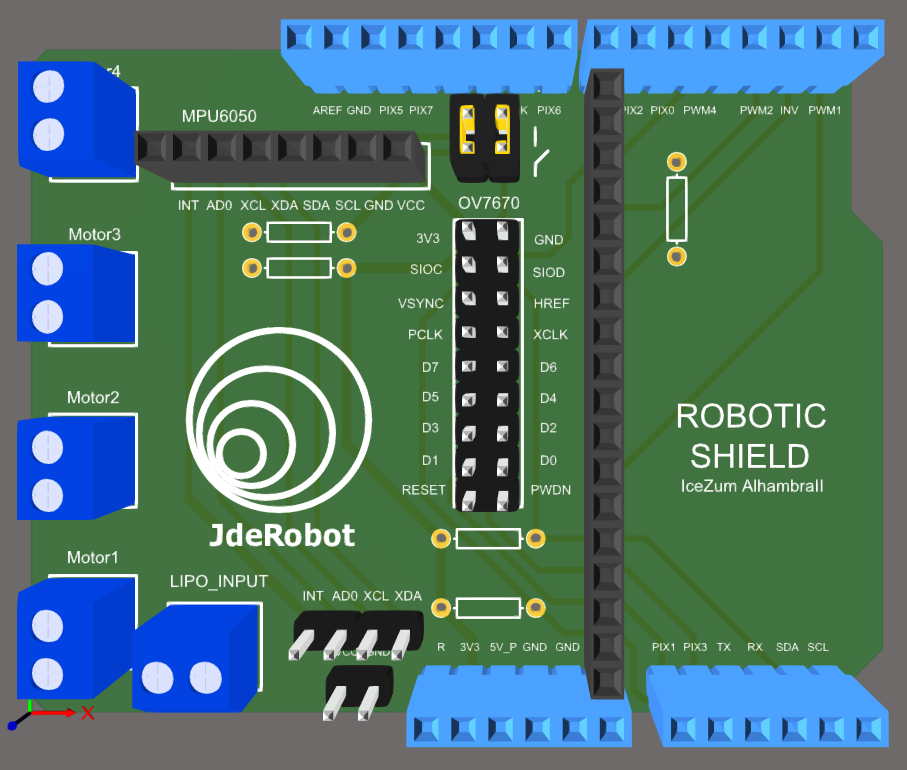
\includegraphics[scale=0.6]{imagenes/Balancing_Robot/top_3D.PNG}
			\caption{3D View of Shield for IceZum Alhambra II.}
			\label{fig:top_3D}
		\end{figure}
	\end{center}
	
	\begin{center}
		\begin{figure}[H]
			\center
			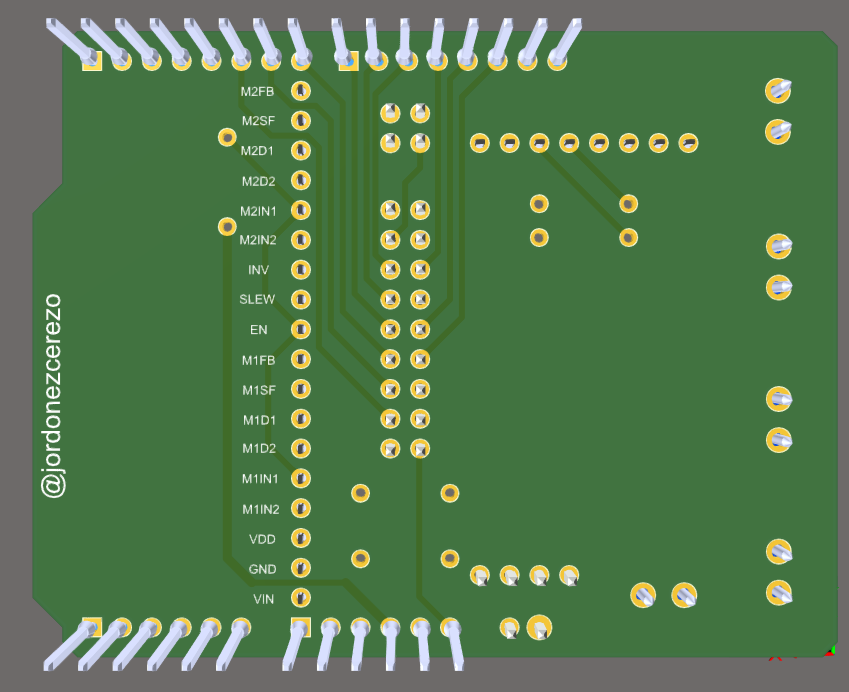
\includegraphics[scale=0.6]{imagenes/Balancing_Robot/bottom_3D.PNG}
			\caption{3D View of Shield for IceZum Alhambra II.}
			\label{fig:bottom_3D}
		\end{figure}
	\end{center}
	
	\begin{center}
		\begin{figure}[H]
			\center
			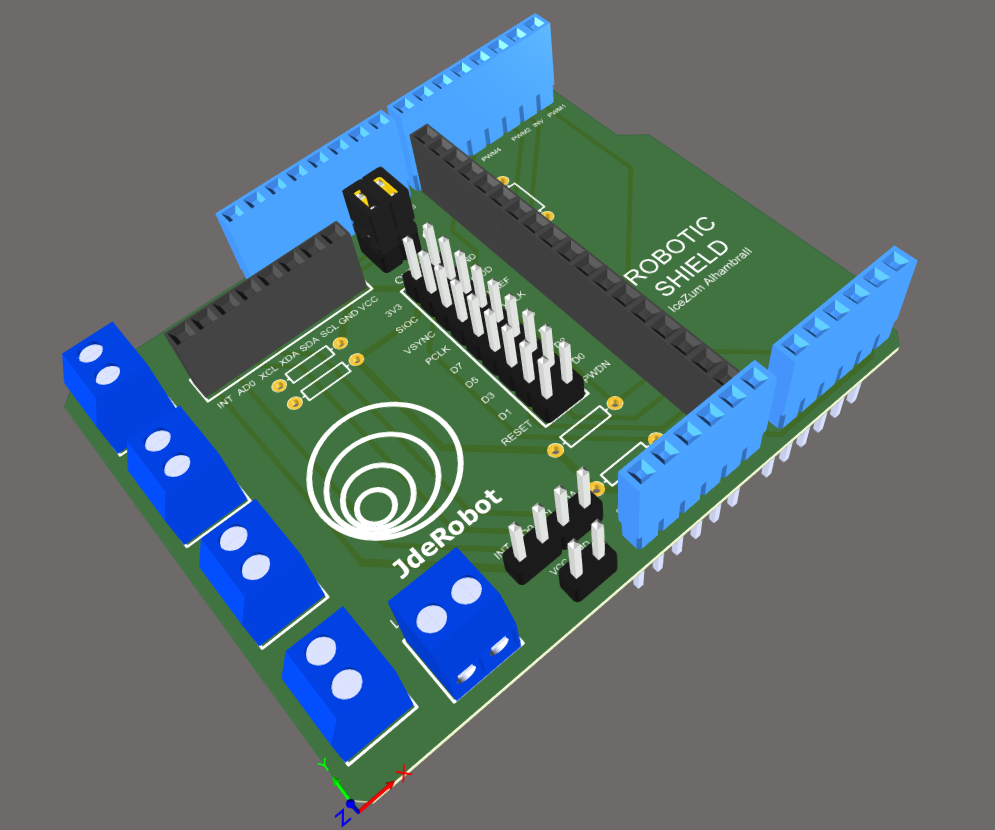
\includegraphics[scale=0.5]{imagenes/Balancing_Robot/Vista3D1.PNG}
			\caption{3D of shield for IceZum Alhambra II.}
			\label{fig:Vista3D1}
		\end{figure}
	\end{center}
	
	\begin{center}
		\begin{figure}[H]
			\center
			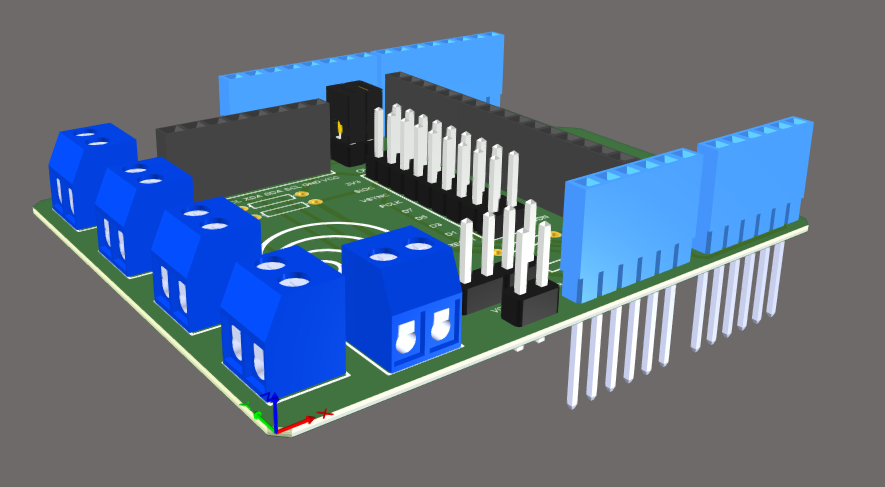
\includegraphics[scale=0.6]{imagenes/Balancing_Robot/Vista3D2.PNG}
			\caption{3D of shield for IceZum Alhambra II.}
			\label{fig:Vista3D2}
		\end{figure}
	\end{center}


For a PCB development with the described requirements it has been used Altium Designer[]. The elaboration process of a PCB in Altium can be different depending on the final user, but in this project the following root has been followed:

\begin{itemize}
	\item At first the project in issue is created.
	\item For each of the components used a new library is created, formed by the schematic and the layout in the PCB.
	\item Once all the libraries are created, the schematic of the plate is designed, taking special care that the connections are adequate.
	\item With the schematic already created, the PCB can be implemented defining its edges, tracks, pads, etc.
\end{itemize}

The scheme is represented in \ref{fig:schematics_tfg}.
\newpage

\begin{center}
	\begin{figure}[H]
		\center
		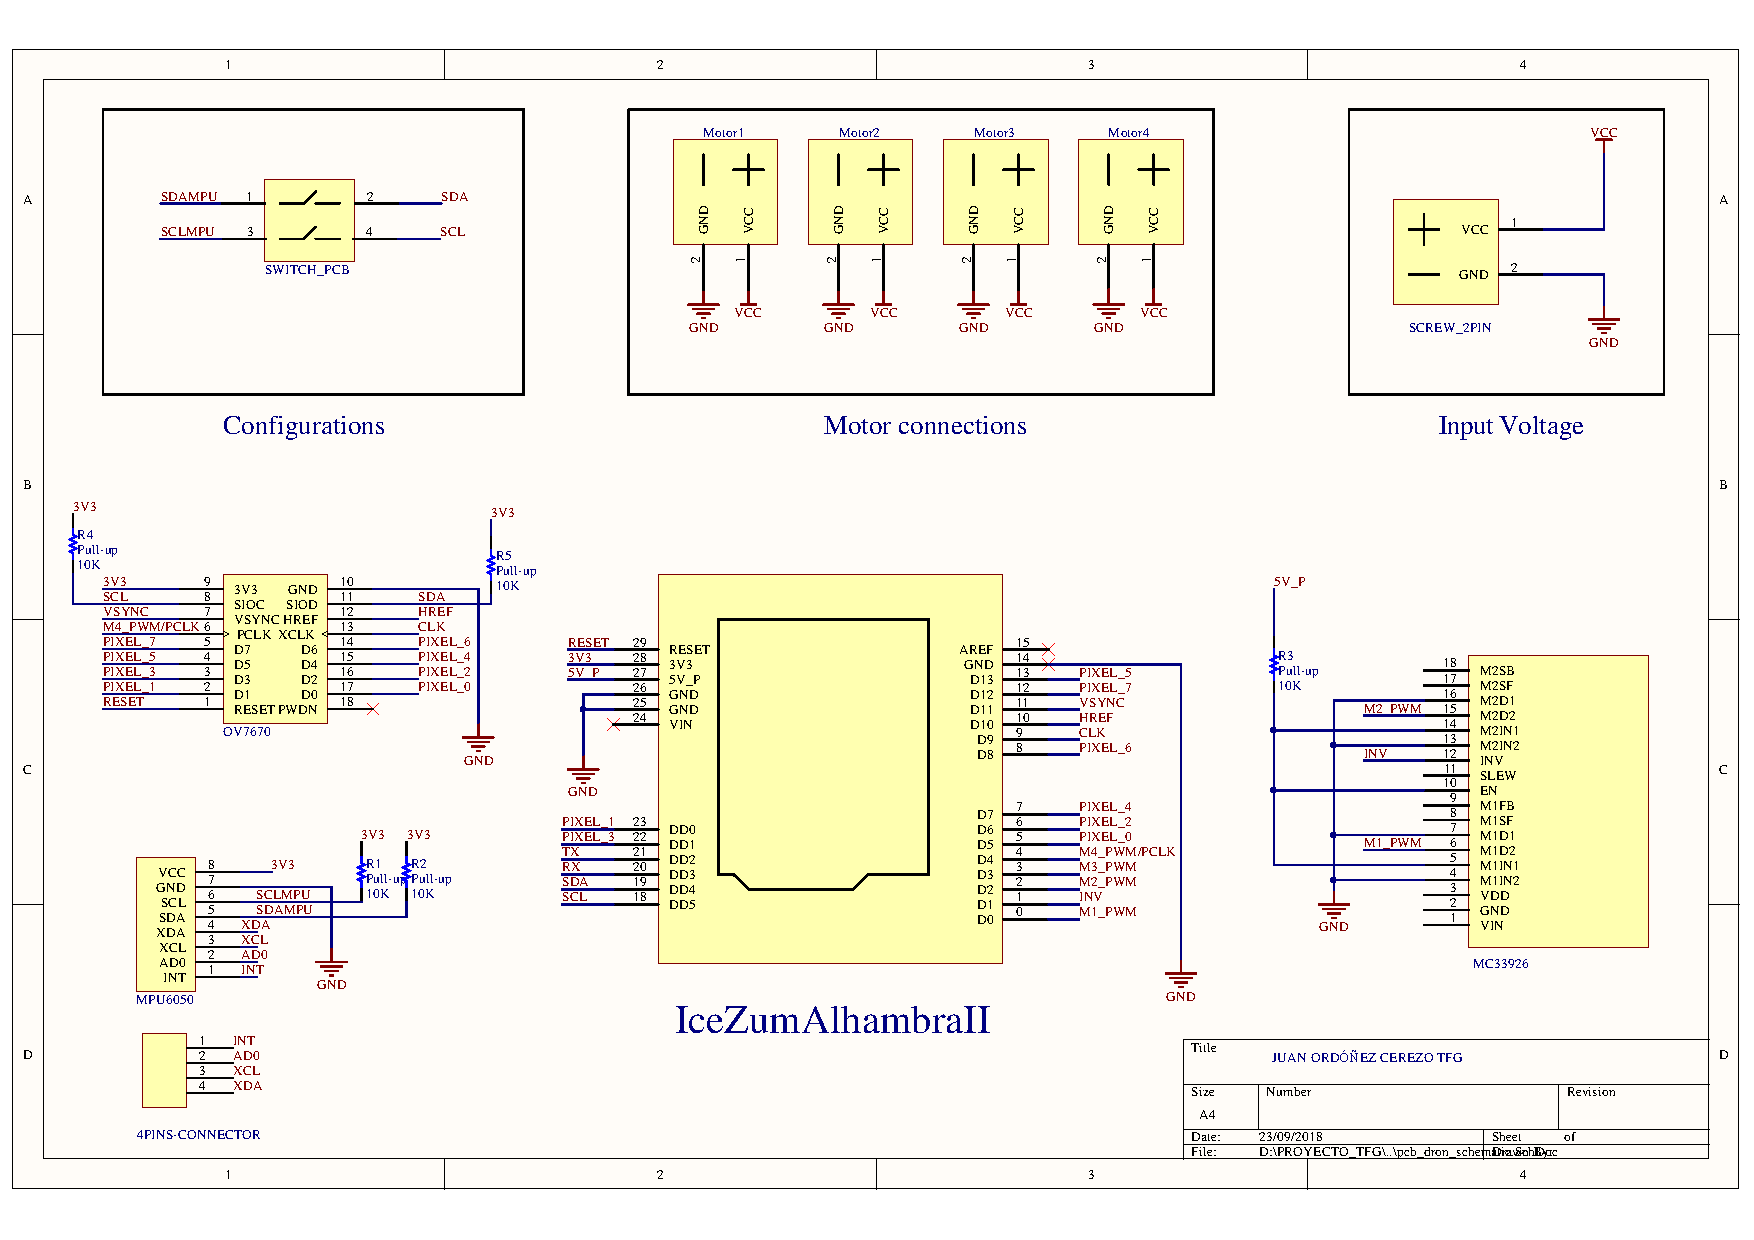
\includegraphics[scale=0.6, angle=90]{imagenes/Balancing_Robot/pcb_dron_schematic.pdf}
		\caption{Schematic Shield IceZum Alhambra II}
		\label{fig:schematics_tfg}
	\end{figure}
\end{center}
\newpage

\textbf{Trace size} \newline
When designing the PCB, the size of the copper trace should be considered, especially if the current could be very high. Otherwise, the PCB could suffer damage or even burn out. \newline

To calculate the trace width, it is necessary first to know the maximum intensity that could circulate through it. It is based on the knowledge that one of the engines of the unmanned aerial vehicle (this is the worst case and for which the calculation of tracks is necessary) can consume a maximum of 20 amps. This amount has been extracted from the datasheet and is usually common for this type of motors. \newline

The formula used to obtain the trace width has been extracted from the standar IPC-2221B[], which establishes the generic requirements for the design of PCB.\newline

The formula is defined as in equation \ref{eqn:eqn31}: 

\begin{equation}
I = K * dT^{0.44}*(W*H)^{0.725}
\label{eqn:eqn31}
\end{equation}

Donde: 
\begin{itemize}
	\item I = Max. Intensity (A).
	\item dT =Temperature rise over ambient (Cº)
	\item W,H = With and Height (mils)
	\item K = 0.024 for internal traces and 0.048 for external traces.
\end{itemize}

The following results were obtained either for inner and outer traces:

\begin{equation*}
W_{externas} = 18.716 mm 
\end{equation*} 
\begin{equation*}
H_{externas} = 	0.035 mm
\end{equation*}
\begin{equation*}
W_{internas} =  48.6876 mm 
\end{equation*} 
\begin{equation*}
H_{internas} = 	0.035 mm
\end{equation*}

The thickness of the layer is provided by the manufacturer. In this project, this web has been used for ordering the PCBs []. \newline 
Trace thickness is commonly measured in "oz" and in this case, the manufacturing company allows a 1oz trace thickness in a PCB with, which is equal to a 0.035mm thickness.\newline
If the results obtained from equation 3.1 are analyzed, the difference between a track in an inner layer and a track in an outer layer is clearly seen.\newline
A PCB is divided into layers, each of the layers has its function and organizing them properly is a good practice to avoid bad behavior. Thus, once the requirements were analyzed, two layers were necessary for the connection of data pins, in addition a ground plane is always recommended in which all the pins connected to GND have a common layer. This avoids noise and interference besides ensuring a good ground reference. \newline
In the used PCB provider, there is no price difference between a three-layer PCB and a four-layer PCB and considering that in the best case the trace width for the brushless motors should be of 1.8716cm, it was reached the determination of the usage of one of the layers as a common plane for the powering traces of the motors. The distribution of the layers would therefore be represented in Table \ref{tabla:layers_altium}.

For the rest of data traces, it is assumed a width of 20 mm, which allows a 1.46 A current, enough for this application.


\renewcommand\tablename{Table}
\begin{table}[H]
	\centering
	
	\begin{tabular}{|l|l|}
		\hline
		Top Overlay           & Overlay              \\ \hline
		Top Solder            & Solder Mask/Coverlay \\ \hline
		\textbf{Top Layer}    & Signal               \\ \hline
		Dielectric 1          & Dielectric           \\ \hline
		\textbf{VCC}          & Signal               \\ \hline
		Dielectric 2          & Dielectric           \\ \hline
		\textbf{GND}          & Signal               \\ \hline
		Dielectric 4          & Dielectric           \\ \hline
		\textbf{Bottom Layer} & Signal               \\ \hline
		Bottom Solder         & Solder Mask/Coverlay \\ \hline
		Bottom Overlay        & Overlay              \\ \hline
	\end{tabular}
	\caption{Layers composition in PCB.}
	\label{tabla:layers_altium}
\end{table}



A 2D image of the Top Layer, VCC, GND, Bottom Layer, Top Overlay and Bottom Overlay layers are shown in Figure \ref{fig:layers_altium}.


\begin{center}
	\begin{figure}[H]
		\center
		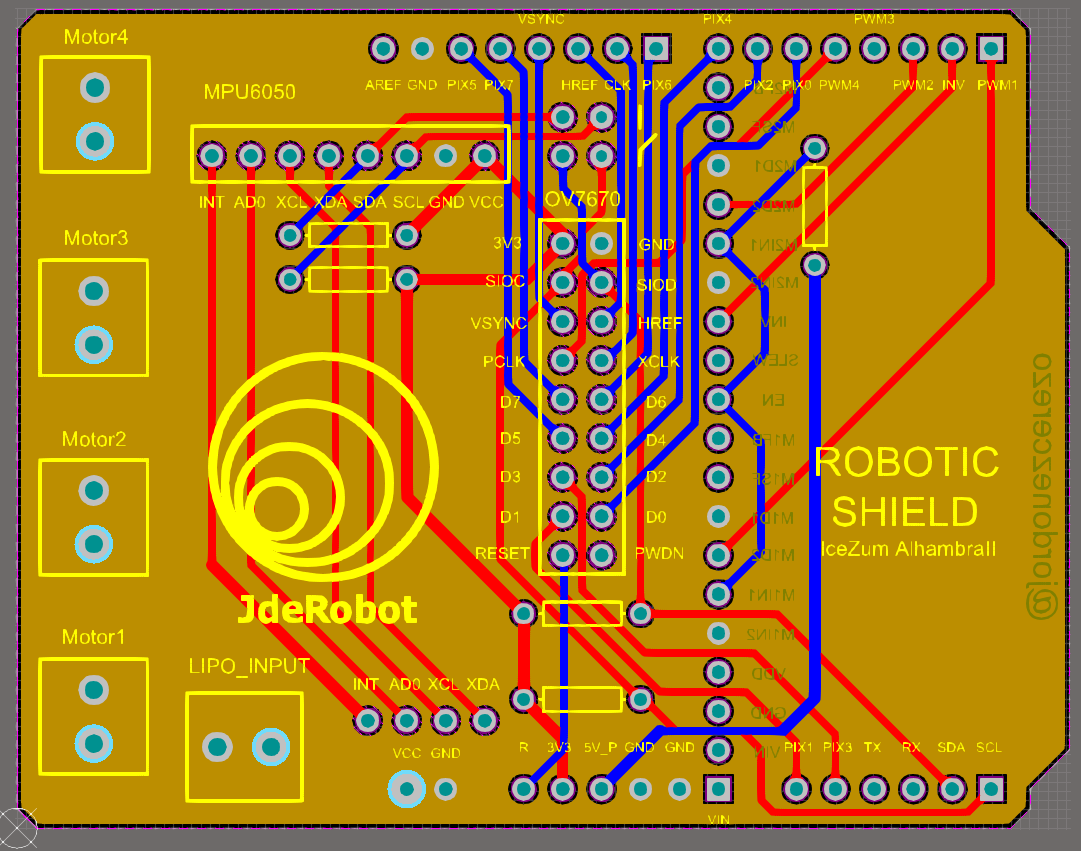
\includegraphics[scale=0.4, angle=90]{imagenes/Balancing_Robot/layers_altium.PNG}
		\caption{Composition layers in Altium.}
		\label{fig:layers_altium}
	\end{figure}
\end{center}


\subsection{IceZum Alhambra-Arduino Nano Implementation}\label{sec:Integracion}

An integration between a microcontroller and FPGA allows to distinguish sequential and parallel tasks, assigning each process to the microcontroller if it necessarily has to be sequential, or to the FPGA if the process can be parallelized and obtain with it some advantages\newline

There are some options to make a Microcontroller/FPGA integration:

\begin{itemize}
	\item Emulate the behavior of a microcontroller in an FPGA.
	\item Physical coexistence of an FPGA and microcontroller creating a communication between each one of them.
\end{itemize}
In this project the second one has been chosen as an option because there are not enough resources to carry out the first one, although this would be the most adequate in terms of saving resources and ease of use. \newline

There are two possible communication types to this purpose:
\begin{itemize}
	\item Serial communication: It is a sequential communication. The bits are sent one by one, sequentially and using only one data bus.
	\item Parallel communication: All bits of each symbol are sent at the same time.
\end{itemize} 

To make usage of the communication in parallel you need as many channels as bits to have the information to be transmitted (if you want to send a byte you should use a total of 8 channels, corresponding to each bit). In this case there will be used 8 pins of the FPGA to be able to carry out this type of transmission. Therefore, and despite the fact that parallel communication is quicker than serial communication, the first one is chosen as the most convenient option. \newline

The type of serial communication developed could be alike an SPI protocol, although it only has data capacity in one direction. The schematic of this developed communication is shown in Figure \ref{fig:coexistencia2}.

\begin{figure}[H]
	\center
	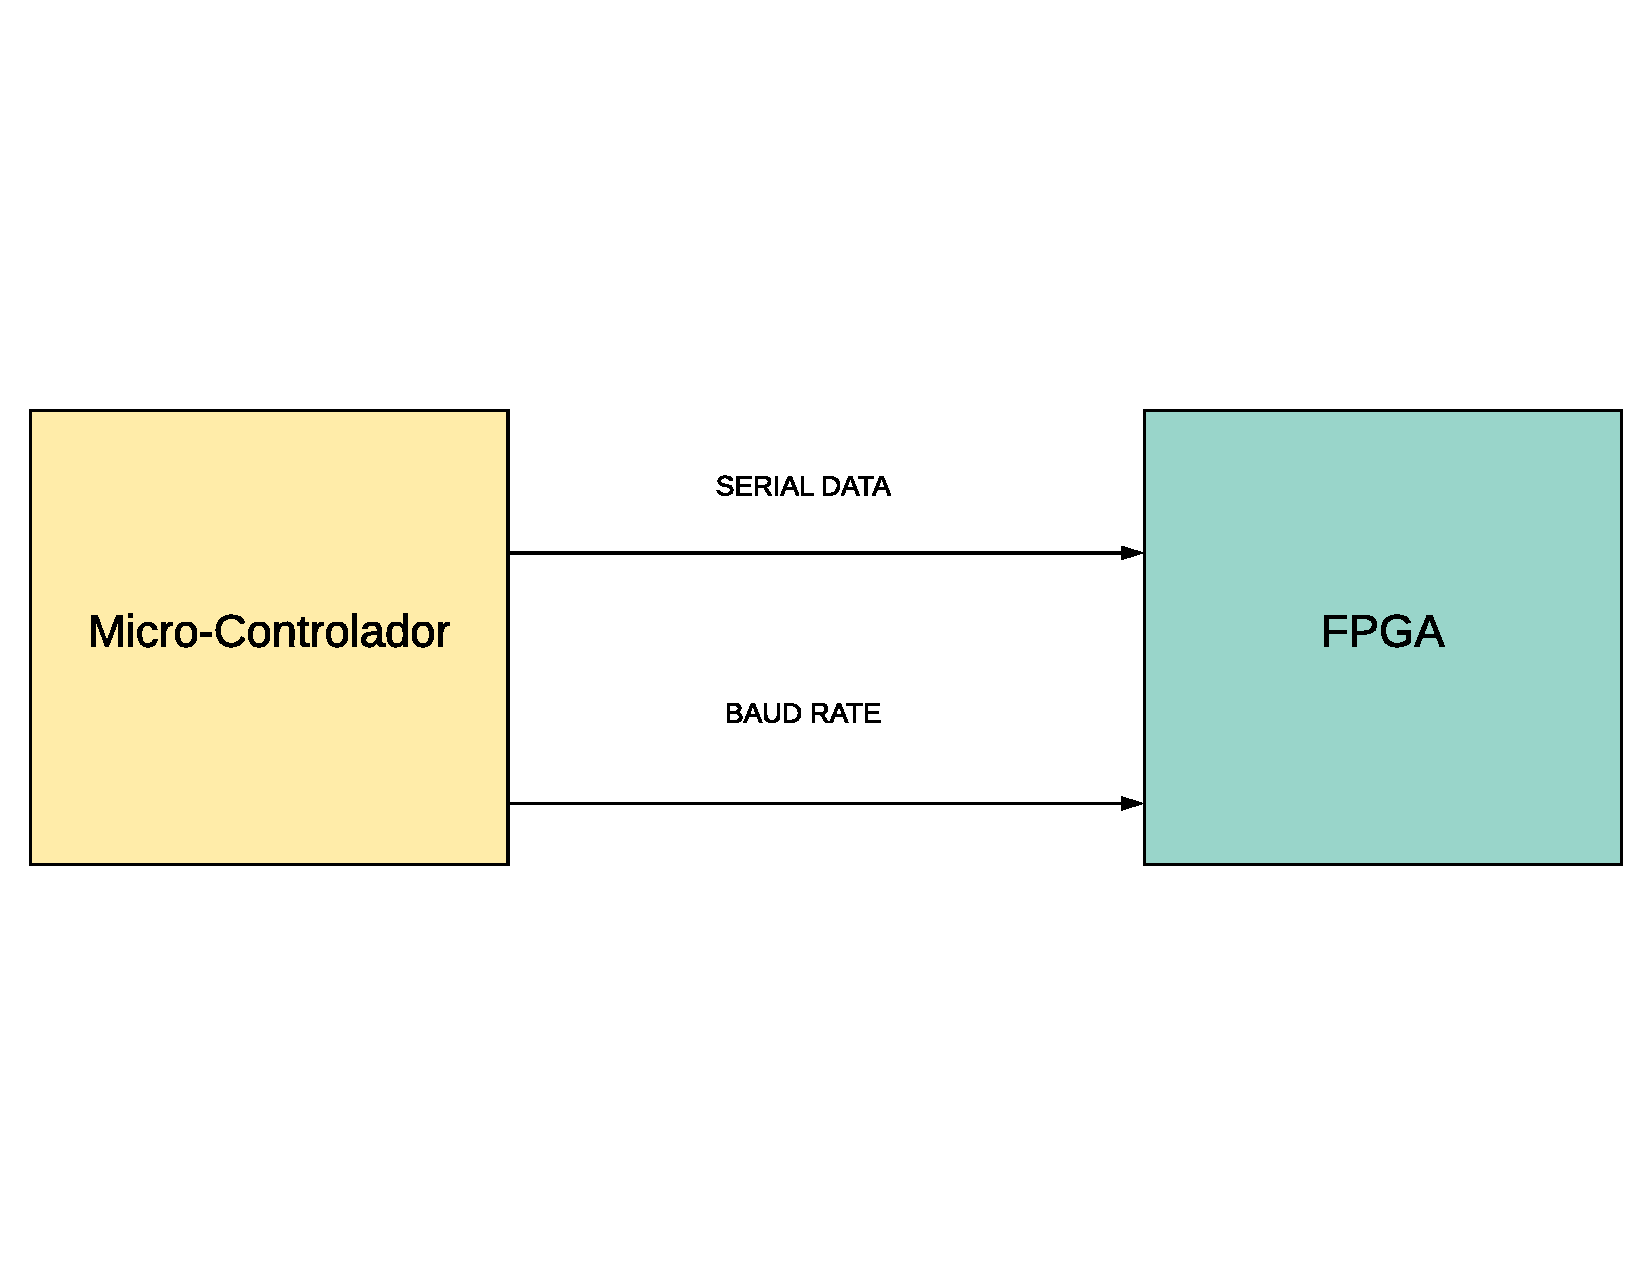
\includegraphics[trim = 0mm 40mm 0mm 20mm, clip,scale=0.4]{imagenes/Balancing_robot/coexistencia2.pdf}
	\caption{Hardware coexistence microcontroller-FPGA.}
	\label{fig:coexistencia2}
\end{figure}
The general system has two connections:
\begin{itemize}
	\item A data line to send the information.
	\item A clock line so that the FPGA could obtain at every time the information speed.
\end{itemize}

A possible example of a serial communication of a data byte could be shown in Figure \ref{fig:serial_comunicattion}. 

\begin{center}
	\begin{figure}[H]
		\center
		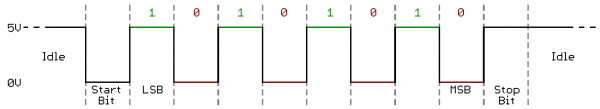
\includegraphics[scale=0.75, angle=0]{imagenes/Balancing_Robot/serial_comunicattion.png}
		\caption{Serial communication example.}
		\label{fig:serial_comunicattion}
	\end{figure}
\end{center}

The angle has to be known in the IceZum-Alhambra in order to make decision both in direction as in the speed of the engines. It is therefore necessary a microcontroller/FPGA communication (Figure \ref{fig:coexistencia1}).

\begin{figure}[H]
	\center
	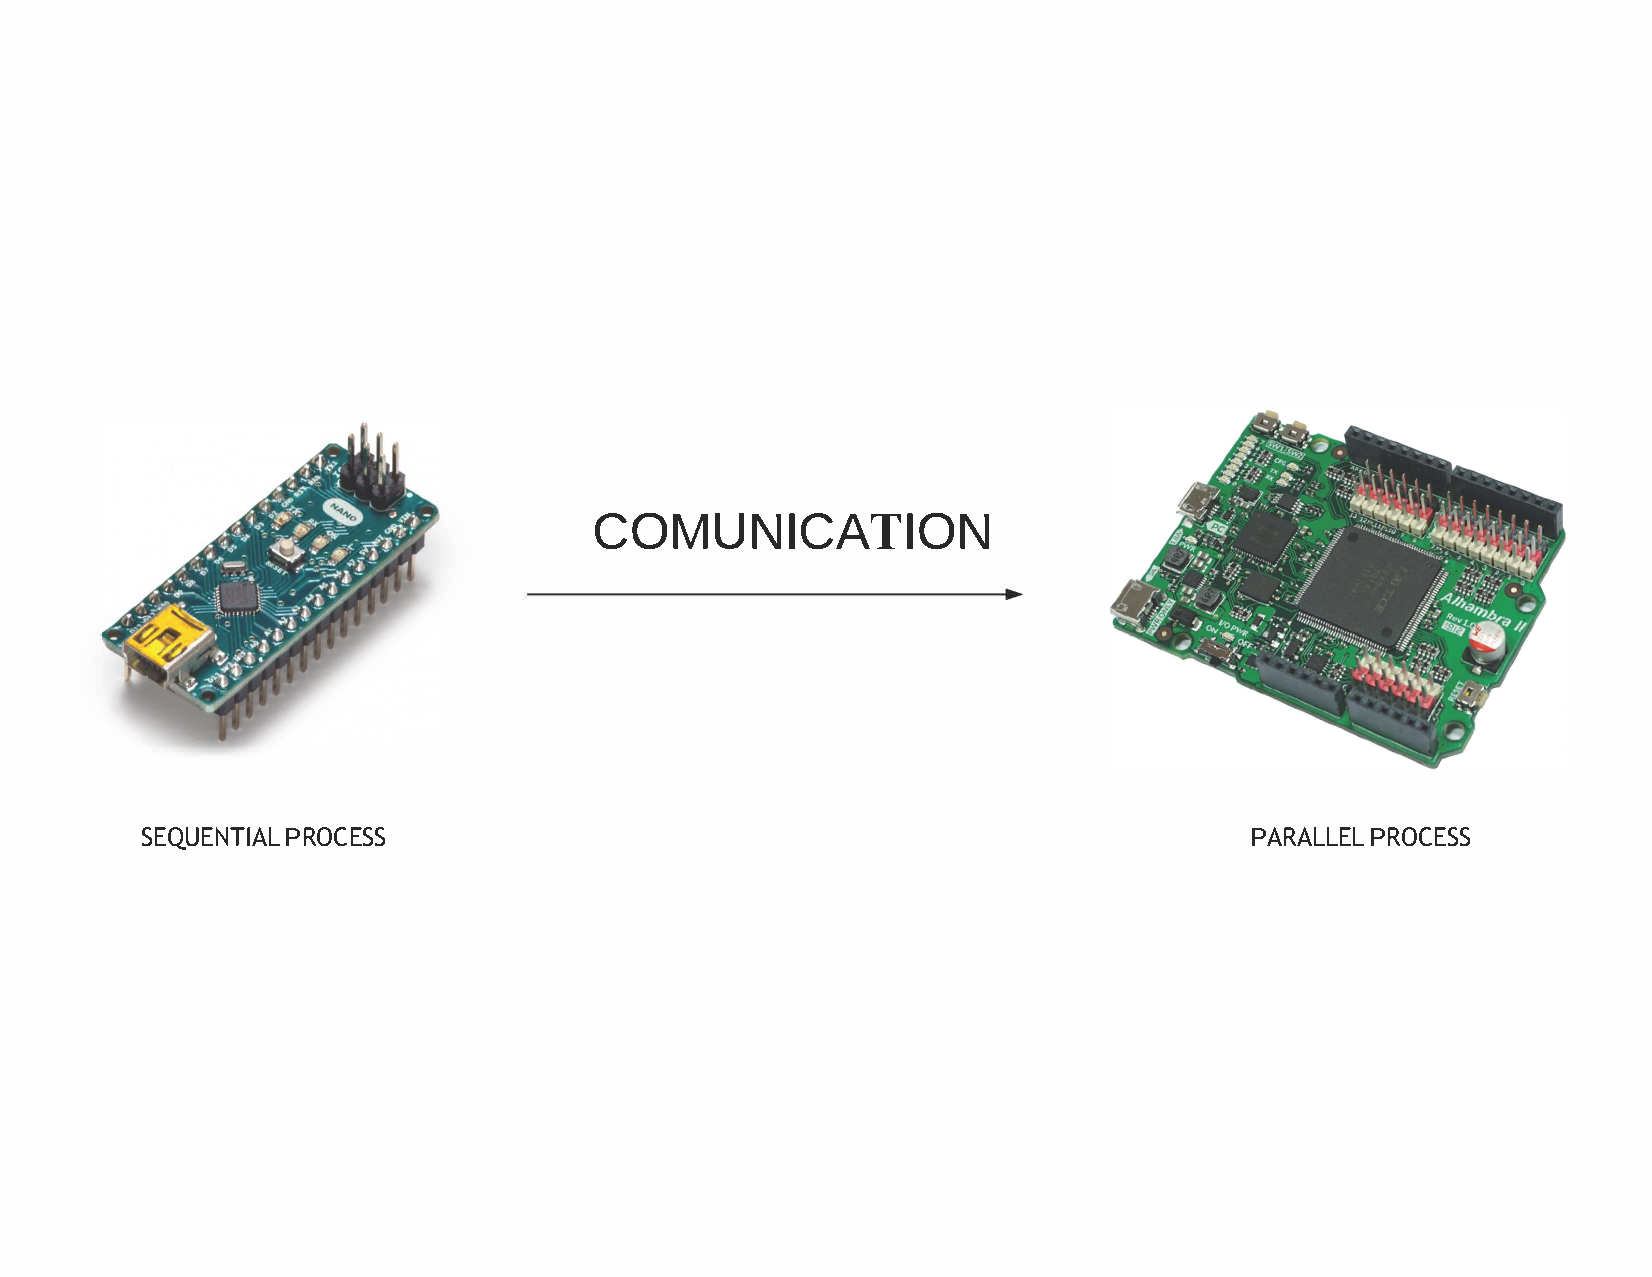
\includegraphics[trim = 0mm 40mm 0mm 20mm, clip,scale=0.4]{imagenes/Balancing_robot/coexistencia1.pdf}
	\caption{Separation microcontroller-FPGA.}
	\label{fig:coexistencia1}
\end{figure}

The communication would be only unidirectional, the microcontroller will send information to the FPGA about the current angle of the object in issue with the purpose that the FPGA analyzes and actuates starting from that angle.\newline

Therefore, there’s a two-part separation: from the point of view of the microcontroller and from the point of view of the FPGA. Both will be explained specifically in subsection \ref{sec:vista_controlador} y \ref{sec:vista_controlador}

\subsubsection{Microcontroller POV}  \label{sec:vista_controlador}

For the development of this sub-chapter, it is assumed that the current angle has already been obtained in the microcontroller. Thus, and for the clarity of the reader, an internal schematic of the Arduino Nano is shown in figure \ref{fig:coexistencia3}. In this section and according to the part of the microcontroller, only the shadowed part is analyzed. 

\begin{figure}[H]
	\center
	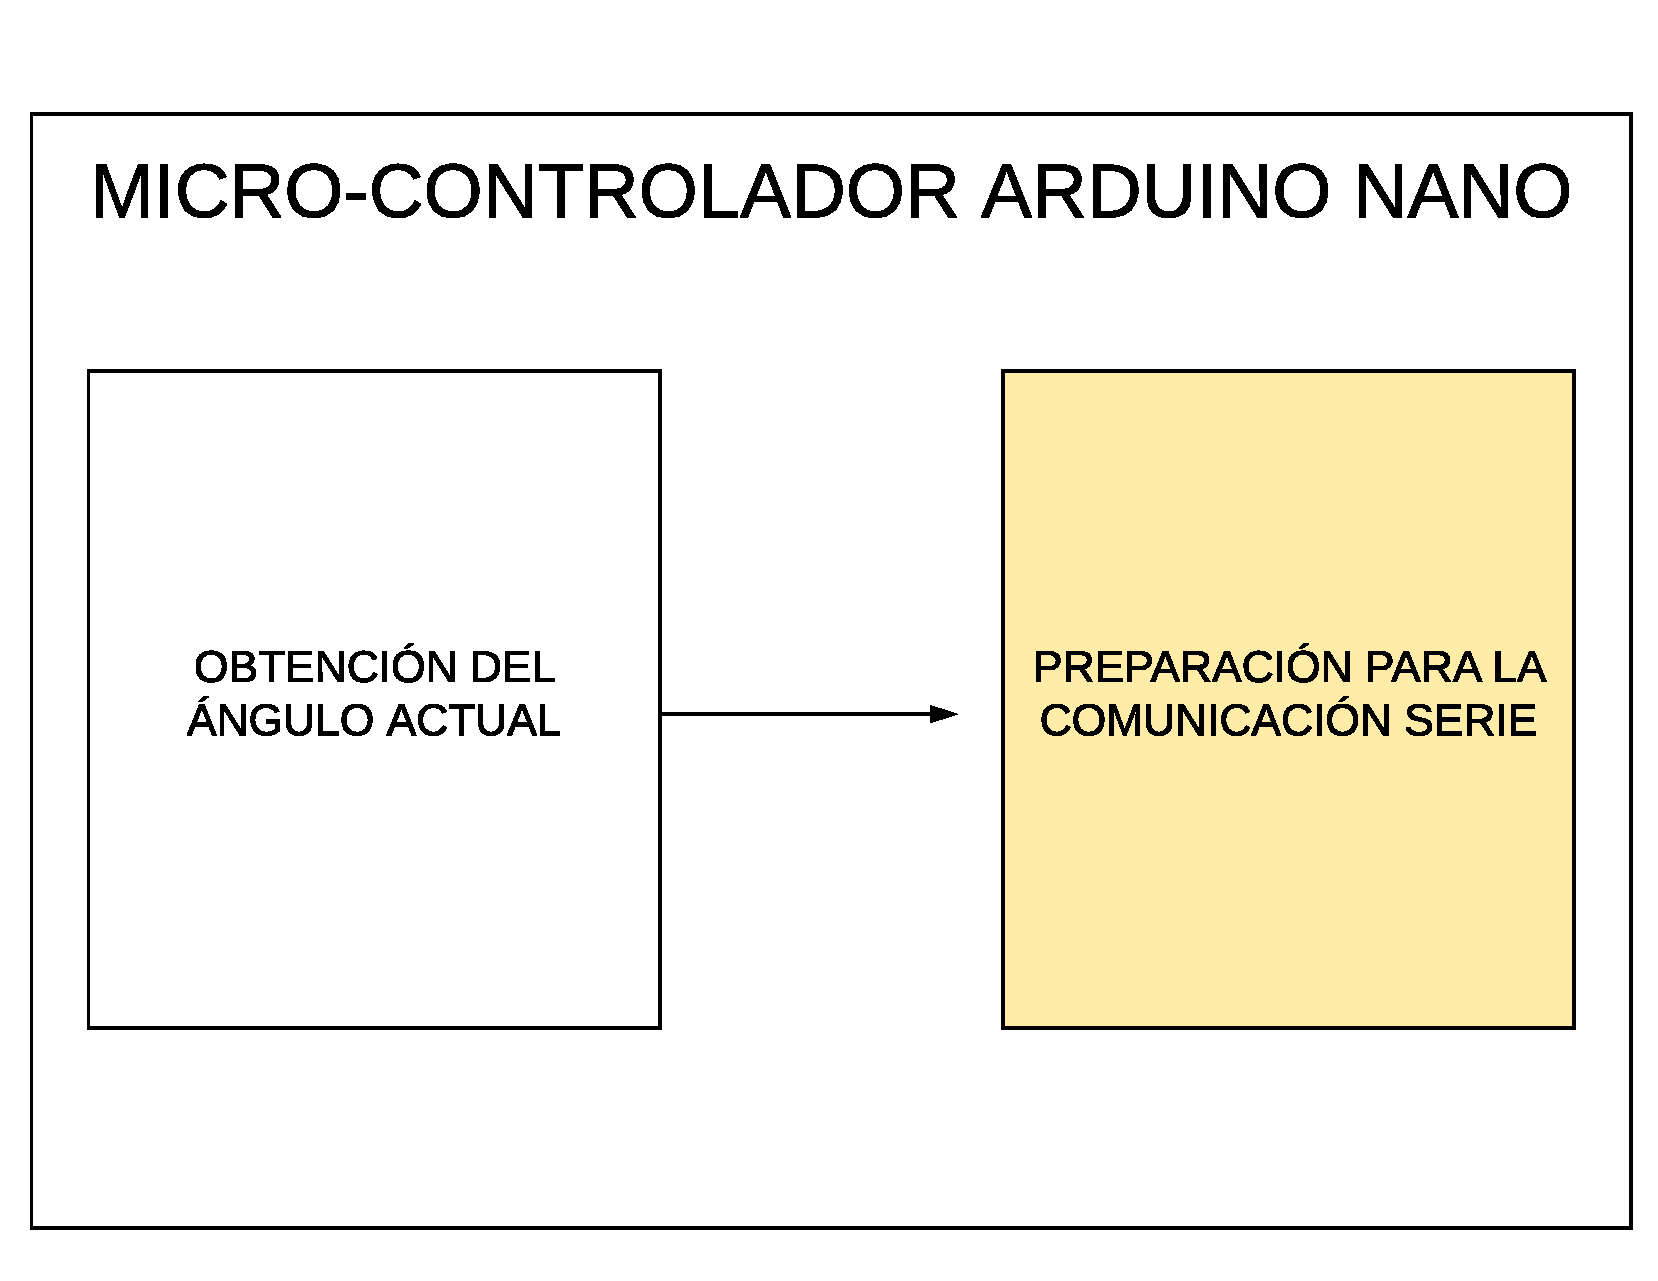
\includegraphics[trim = 0mm 0mm 0mm 0mm, clip,scale=0.3]{imagenes/Balancing_robot/coexistencia3.pdf}
	\caption{Inner diagram Arduino Nano.}
	\label{fig:coexistencia3}
\end{figure}

The flow diagram in which the C code of the microcontroller is based on, is shown in Figure \ref{fig:extraccion_angulo}.

\begin{figure}[H]
	\center
	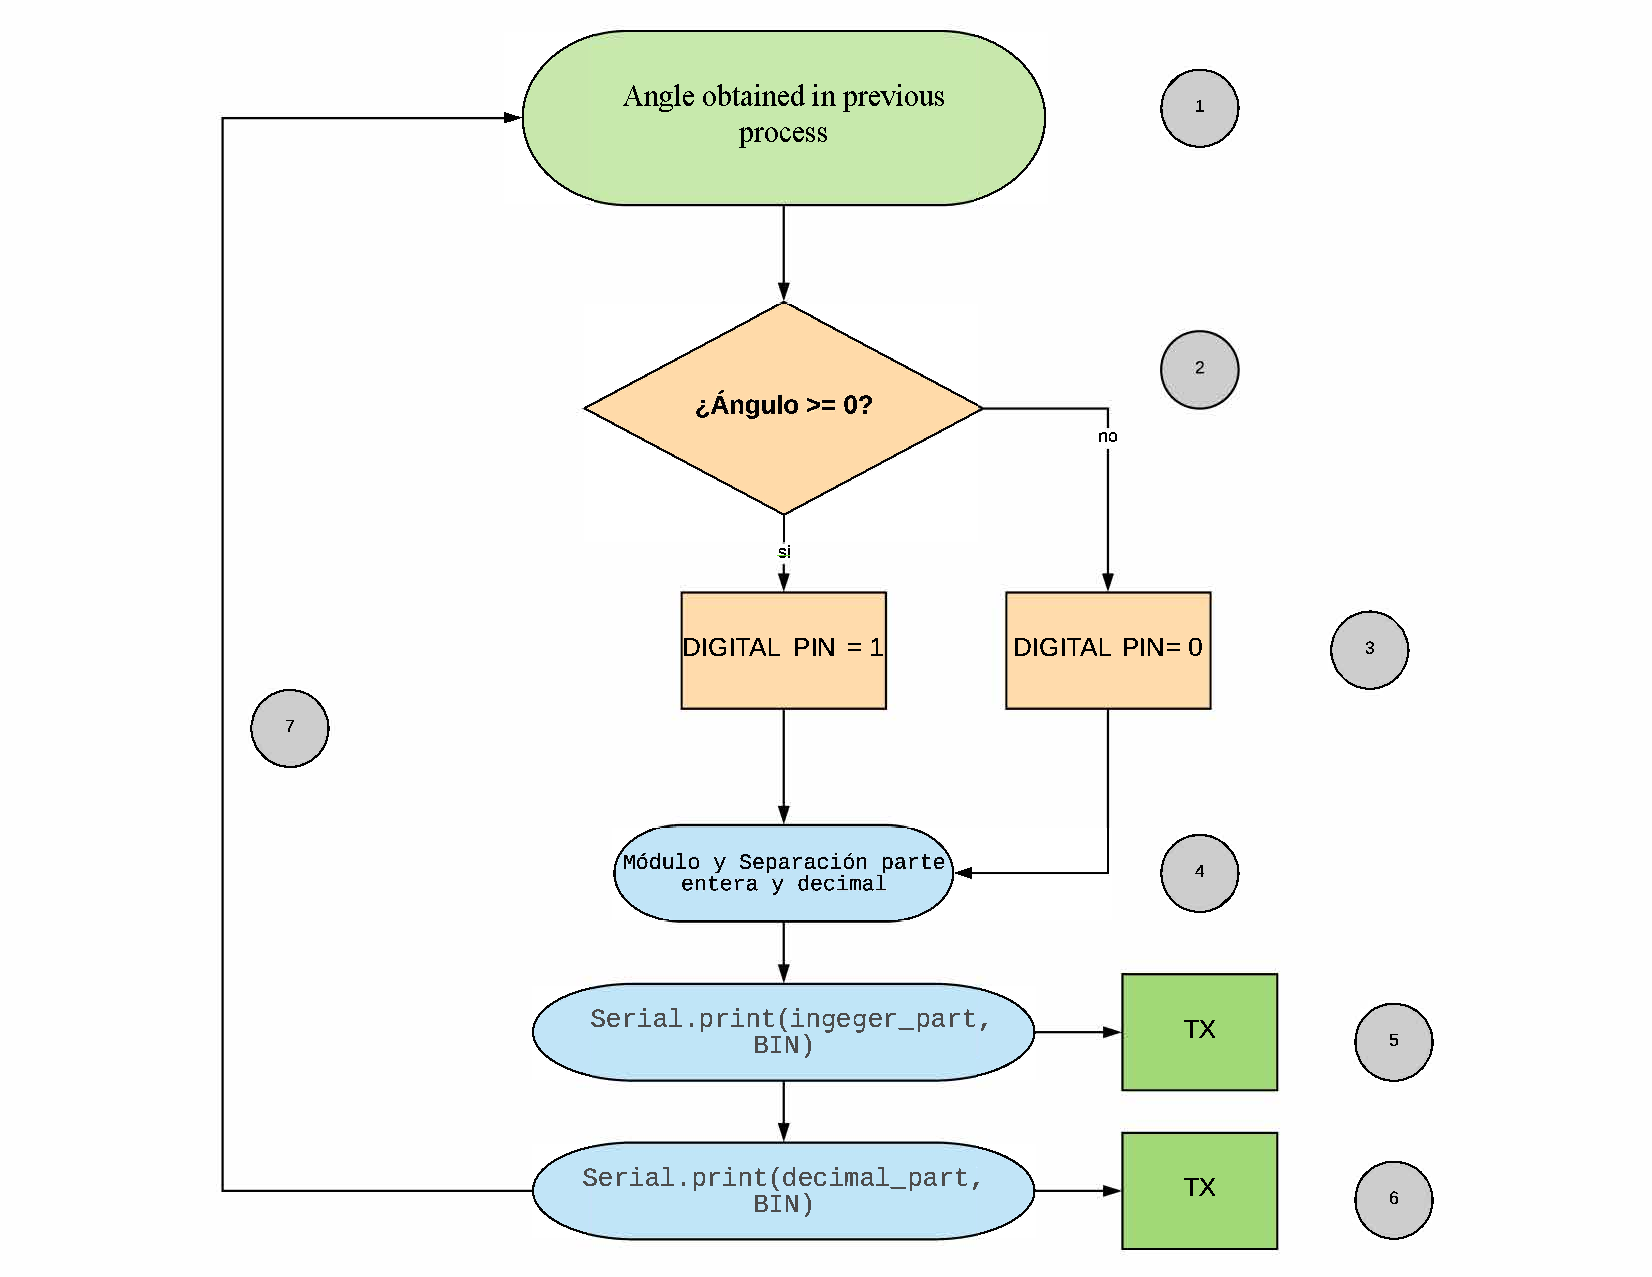
\includegraphics[trim = 0mm 0mm 0mm 0mm, clip,scale=0.5]{imagenes/Balancing_robot/extraccion_angulo.pdf}
	\caption{Flow diagram to send angle.}
	\label{fig:extraccion_angulo}
\end{figure}

The most relevant features will be explained: 

\begin{itemize}
	\item It is based on the assumption that the angle has already been obtained and is correct. In section \ref{sec:MPU6050} you can find more information about it.
	\item As it has been said before 3.3.2, one of the most important parts to correct the control of the self-balance robot, is to know the inclination at every moment to correct this desviation (\ref{fig:angle_correction}). To do this, the FPGA must know if the angle is positive or negative. This aspect would not form part of the communication protocol itself, as will be seen below. 
\end{itemize}
	
	\begin{figure}[H]
		\center
		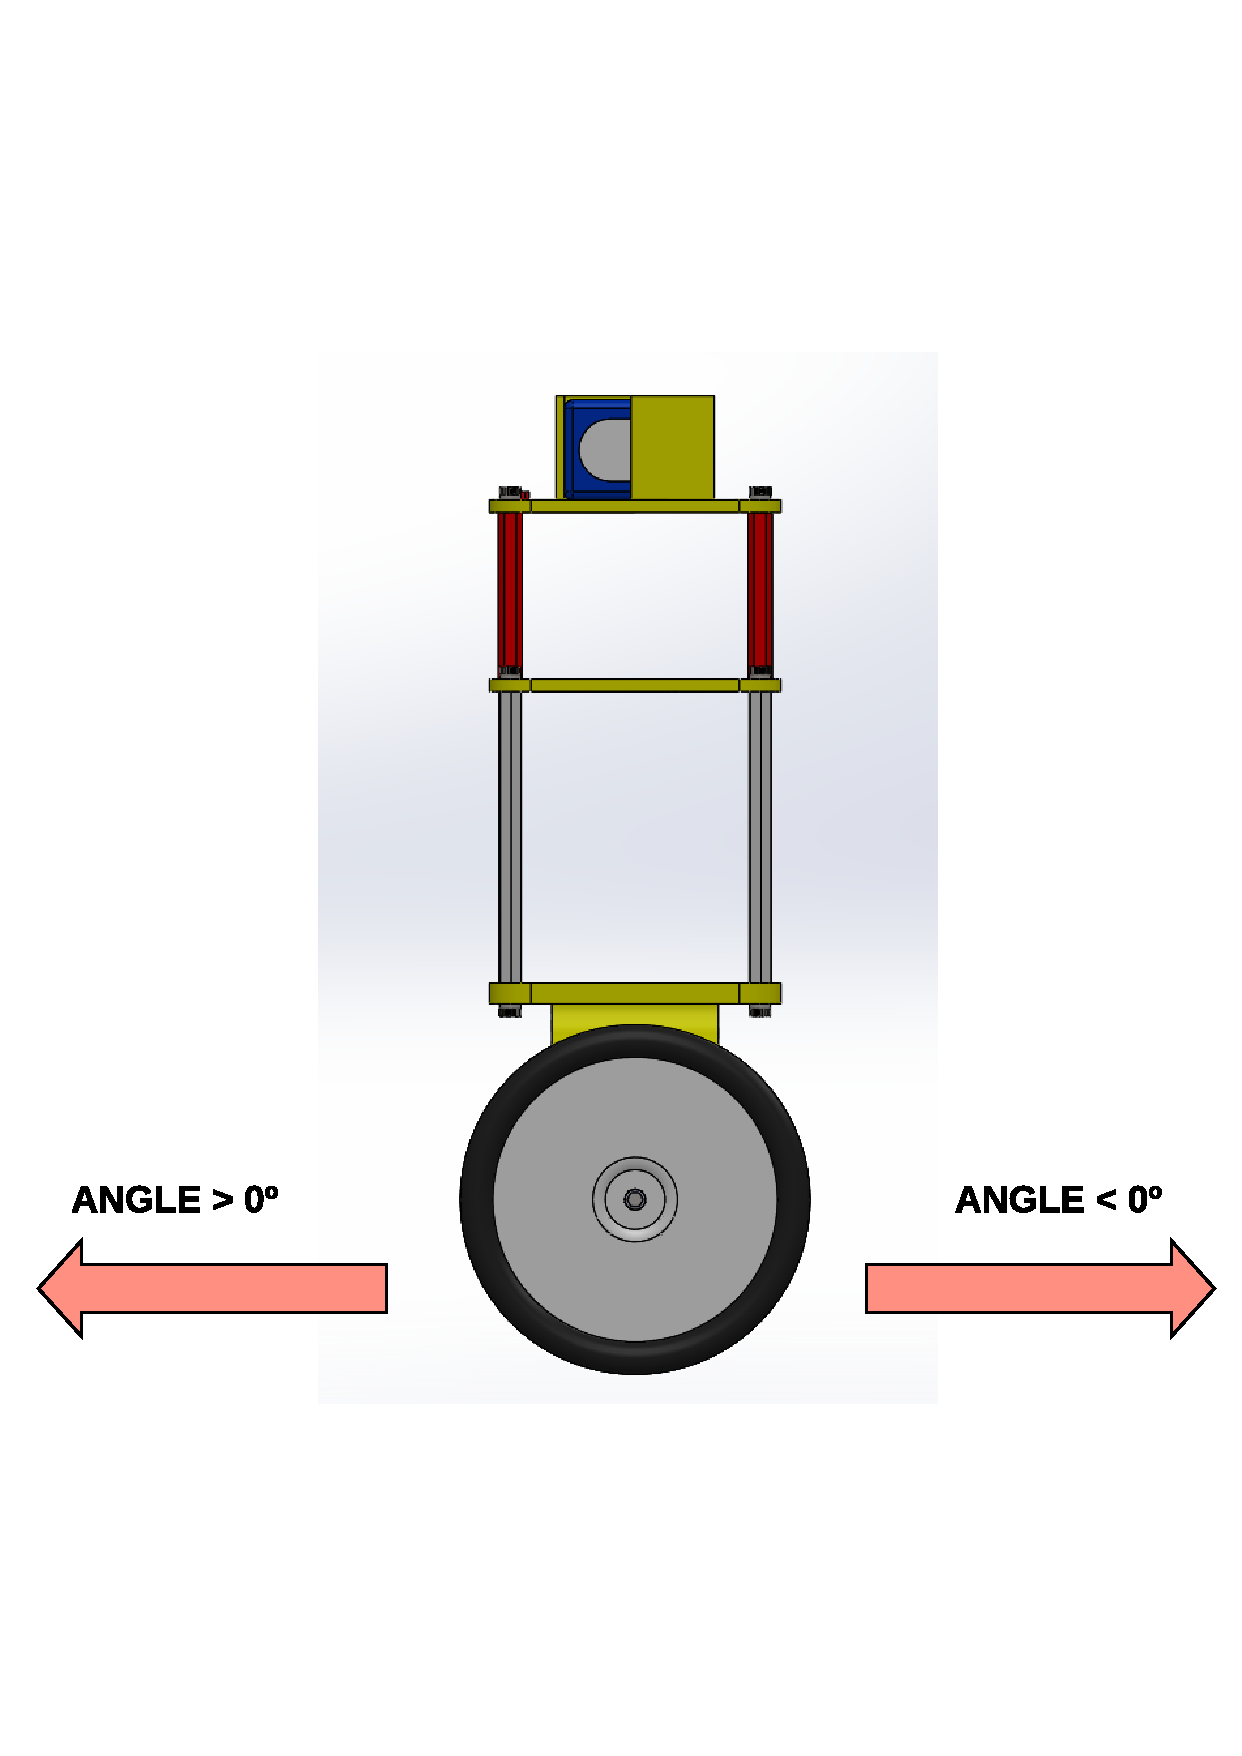
\includegraphics[trim = 0cm 4cm 0mm 4cm, clip,scale=0.5]{imagenes/Balancing_robot/angle_correction.pdf}
		\caption{Correction angle in Self-Balance Robot.}
		\label{fig:angle_correction}
	\end{figure}
	
\begin{itemize}	
	\item A single pin of the microcontroller is used, which will change its value to 1 or 0 depending on the sign of the angle at each moment. This way the FPGA will only have to read this information when it is necessary.
	
	\item For a correct understanding by the FPGA it is necessary to send the represented Angle in bytes and not in ASCII code. This is why for that sending the "Serial.print(Angle)" command will be used. This Arduino function sends by the serial port the representation in bytes of the angle in issue.\newline
	If the whole angle is intended to be sent, both the symbol and the ASCII code of the comma will be sent, and this is an aspect that does not matter to be considered when processing the FPGA is referred. To correct it, first the module of the angle is made (the sign is not needed because there is already a pin designated for it) and later it makes a separation between the integer and the decimal part in order to eliminate the "comma" character.
	\item The integer part corresponding byte is sent by the serial port.
	\item The decimal part corresponding byte is sent by parallel port.
	\item This is a loop that will be reproducing each “x” seconds, this is, the angle that could be corrected each “x” seconds. 
\end{itemize}
A real example of the angle being sent with its corresponding sign is shown in the following Figure: \ref{label}

\textbf{captura del envio del angulo}

\subsubsection{FPGA POV} \label{sec:vista_fpga}

For an input PIN to the FPGA it will be continuously entering data from the transmission pin and so that it can make a correct reading of the byte it is necessary to know: 

\begin{itemize}
	\item When a byte transmission starts.
	\item When a byte transmission ends.
	\item When a bit can be captured. 
	\item When the necessary bits are saved in a buffed until the byte is complete.
\end{itemize}

In order to implement an intermediate module in the FPGA with the previous features (aspect in IceStudio Figure \ref{fig:arduino_interface}) it is necessary previously know the speed of the transmission by the microcontroller, which has been 16200 baud. \newline


\begin{figure}[H]
	\center	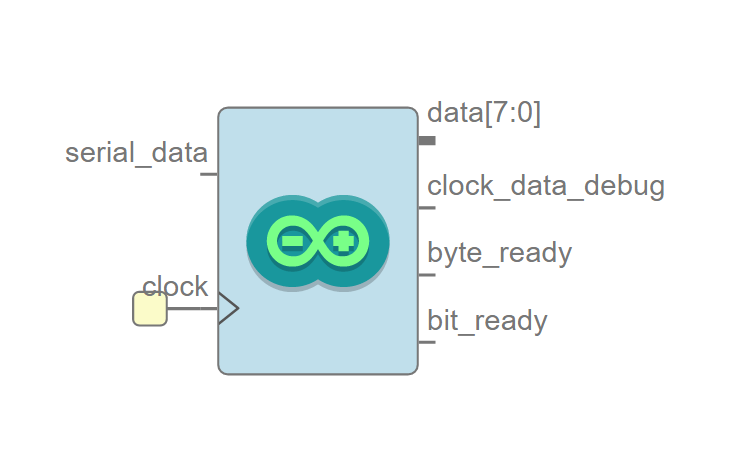
\includegraphics[scale=0.6]{imagenes/Balancing_robot/arduino_interface.PNG}
	\caption{Appearance of 	Arduino Nano module in IceStudio.}
	\label{fig:arduino_interface}
\end{figure}

The inputs and outputs from the previous module are detailed:

\begin{itemize}
	\item data[7:0]:Consists in a buffer in which bits are being stored when it is necessary until we have the byte. It is important that the following module knows when the byte is prepared for its capture.
	\item clock\_data\_debug: The usage of this output is for depuration only.
	\item byte\_ready: A clock flag will change its state when a byte is ready to be captured. As there has been seen in previous developments, this byte will be both integer or decimal part.
	\item bit\_ready:The usage of this output is for depuration only.
\end{itemize} 

The implementation in IceStudio of the previous behavior is implemented by two machine states with their corresponding sensitivity lists and the flow diagram is represented in Figure \ref{fig:arduino_interfacefluid}.

\begin{center}
	\begin{figure}[H]
		\center
		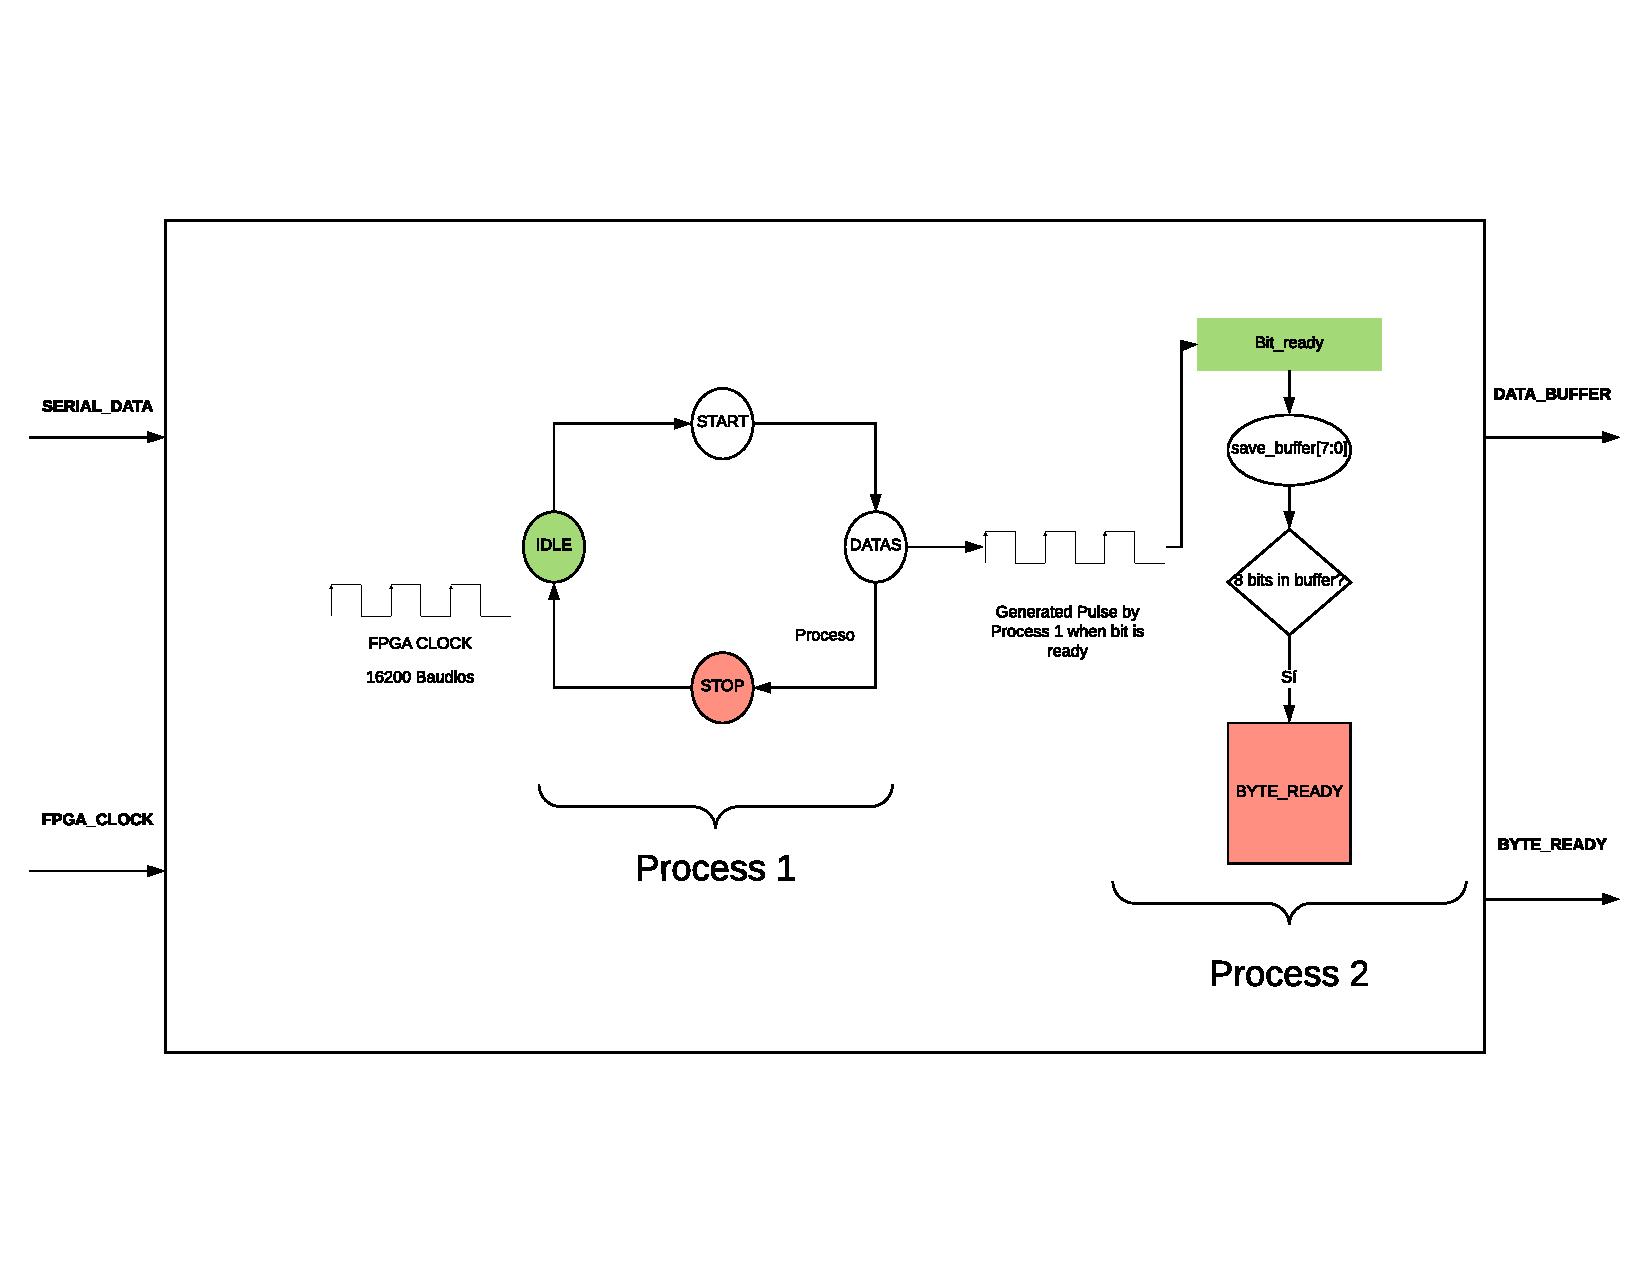
\includegraphics[trim = 0mm 0mm 0mm 10mm, clip,scale=0.7, angle=90]{imagenes/Balancing_robot/arduino_interfacefluid.pdf}
		\caption{Flow diagram for Arduino interface.}
		\label{fig:arduino_interfacefluid}
	\end{figure}
\end{center}

 Two well differenced processes are used:\newline
\textbf{Process 1:} This process only gives the next system the exact moment at which it can
capture a bit and save it in the buffer, for this, you must know the speed of the transmission discussed above. The states would be the following:

\begin{itemize}
	\item IDLE: The process remains in this state until the transmission starts, which will go to the next state (START).
	\item START: How was it developed in the section … The serial transmission protocol begins with a start condition, this state will allow to recognize when this condition ends to start saving bits in the buffer. 
	\item DATA: Since the transmission speed is already known and the condition of START in the previous state has been recognized, in this state a flag will change its value
	when the bit is ready to be stored in the buffer, of which process 2 will be in charge of.
	\item STOP: In addition to a START condition, the serial transmission protocol used in Arduino has a STOP condition. This state allows to recognize the time it takes Arduino to carry out this last condition, then, it will return to the first state until a new transaction begins.
\end{itemize}

\textbf{Process 2:} This process activated by process 1. When process 1 determines that a bit is available on the bus to be captured, it will set a clock flag on, initiating process 1 through a sensitivity list. The flow diagram could be:

\begin{itemize}
	\item Wait until the sensibility list is activates, this will indicate that a bit could be captured.
	\item Bits will be storing in a buffer that will form a byte, which will represent the integer or decimal part of the angle at that moment.
	\item When the byte is prepared to be captured by two consecutive modules, a channel will be on, being available both the outputs and the buffer with the 8 bits and the channel "byte\_ready".
\end{itemize}

At this point the FPGA is able to differentiate when it can capture a byte (BYTE\_READY) and from where it has to capture the data bus (DATA\_BUFFER). However, an aspect that is not part of the communication itself, it is important to analyze if you want to get a correct operation. That is, if it has been previously said that the microcontroller continuously sends the integer and decimal part of the angle, if a good interpretation of this data is not made, it is possible that an angle on the FPGA is formed by a decimal part of an angle \textit{n} and the integer part of the angle \textit{n + 1}.  \newline

To do this, a module is created in IceStudio that is capable of ordering these values. The aspect of this module in IceStudio is shown in Figure 3.29. \ref{fig:arrange_arduino}.

\begin{figure}[H]
	\center
	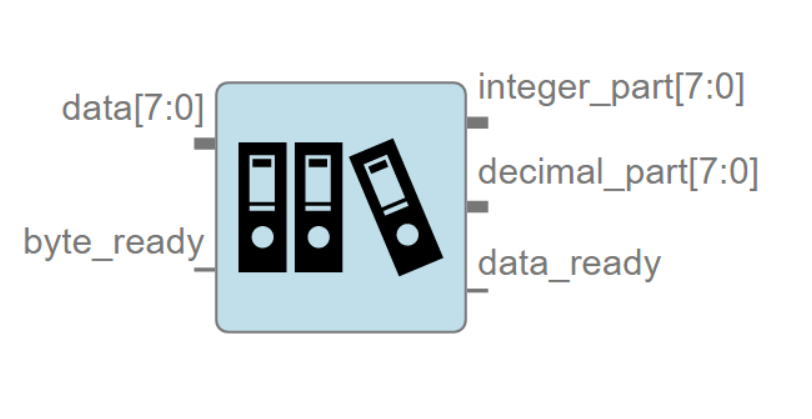
\includegraphics[scale=0.4]{imagenes/Balancing_robot/arrange_arduino.PNG}
	\caption{Module to arrange data from Arduino.}
	\label{fig:arrange_arduino}
\end{figure}

As Inputs there are:

\begin{itemize}
	\item Data [7:0]: This is the output buffer of the previous module where all captured bits are being stored until the byte is completed.
	\item byte\_ready : Clock flag which activates when the byte is available to be captured.
\end{itemize}

It is important to consider that the data will be available as long as the entire part as well as the decimal part of the angle in issue is available. Thus, as outputs are:

\begin{itemize}
	\item integer\_part[7:0] :Byte that represents the integer part of the angle.
	\item decimal\_part[7:0] : Byte that represents the decimal part of the angle.
	\item data\_ready : Clock flag that activates when the data (decimal and integer part) is waiting to be captured.
\end{itemize}

As has been previously discussed, the flow diagram of the code in Verilog that implements the previous behavior is shown in Figure \ref{fig:arrange_angle}.

\begin{figure}[H]
	\center
	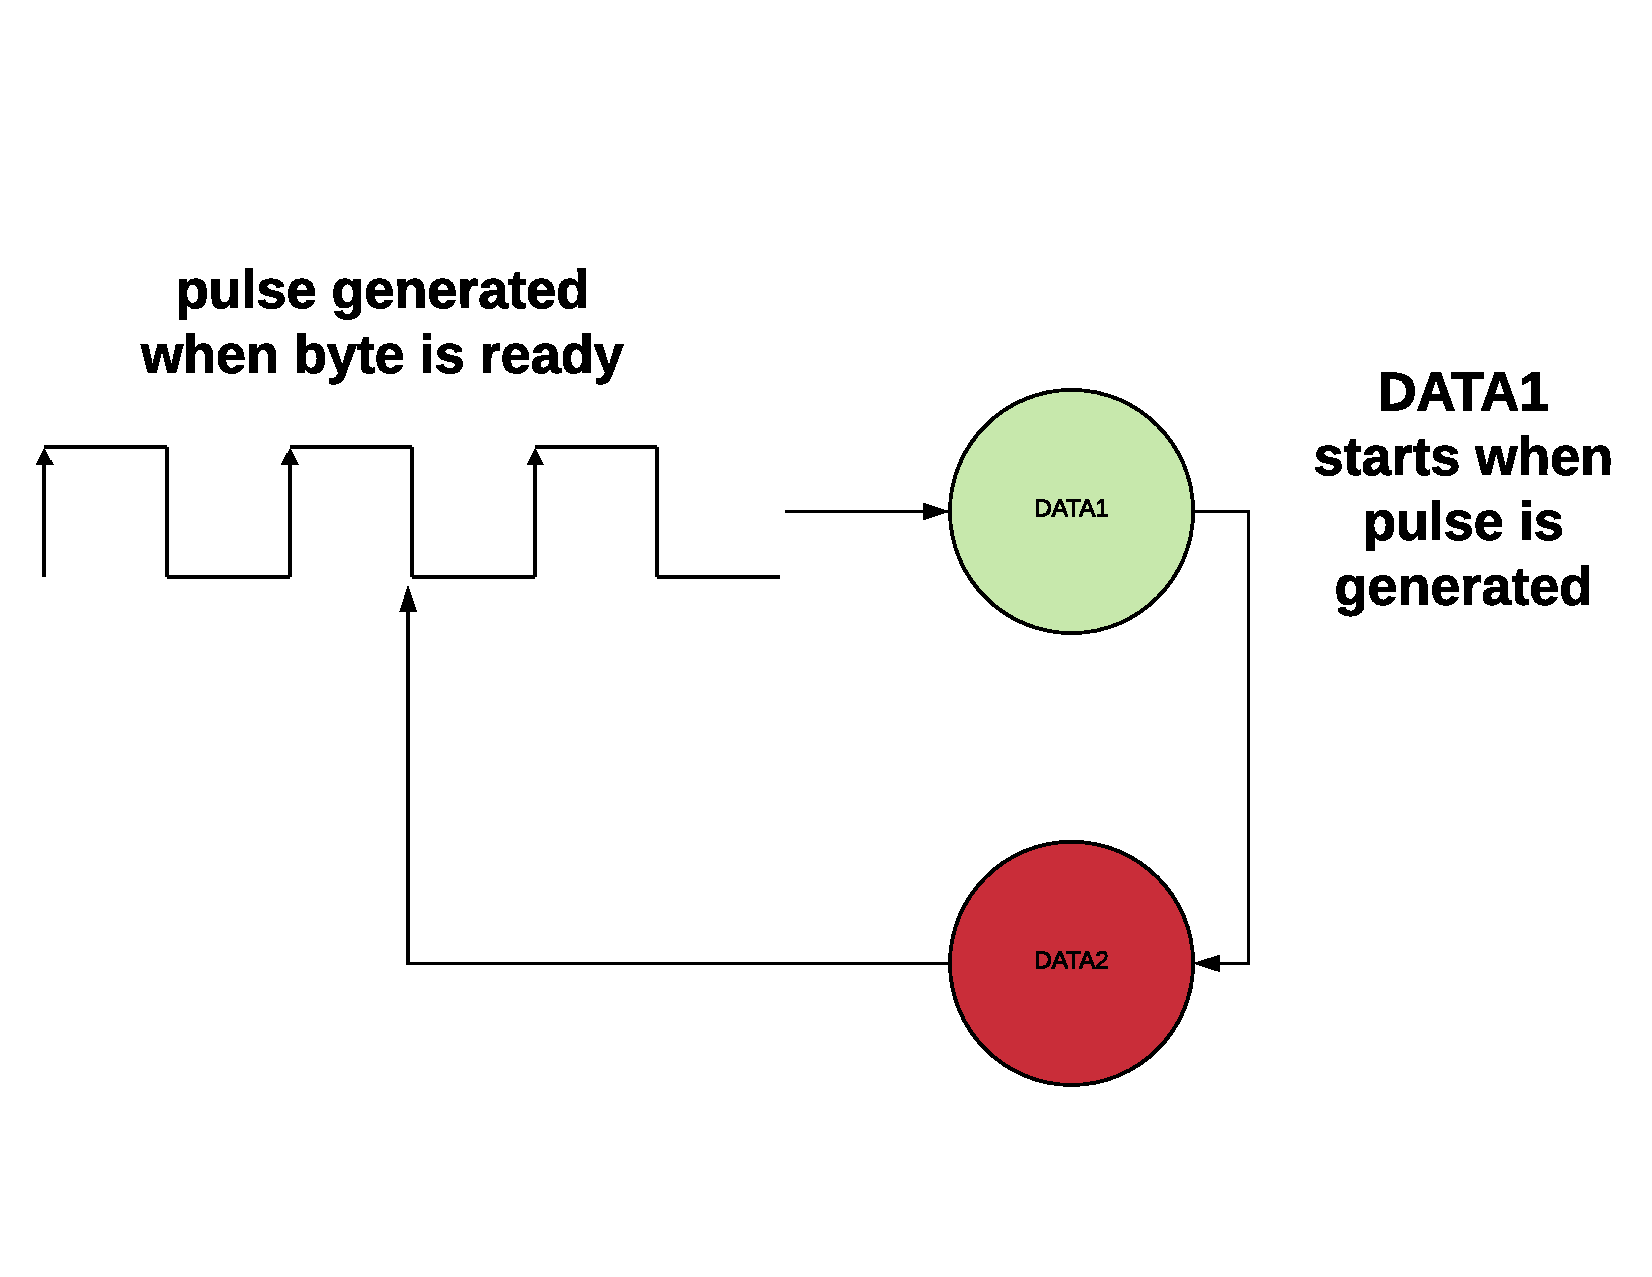
\includegraphics[[trim = 0mm 4cm 0mm 4cm,clip, angle=0,scale=0.4]{imagenes/Balancing_robot/arrange_angle.pdf}
	\caption{Flow diagram to arrange bytes.}
	\label{fig:arrange_angle}
\end{figure}



In this case is a process with a sensibility list that counts as a sensible signal the "byte\_ready", bus and which is the output from the previous module. \newline

Each time the flag is activated that indicates that a byte Is ready to be captured, a cyclic state machine starts that counts with the following states:

\begin{itemize}
	\item DATA1: It is the first data to be captured and corresponds to the whole part of the first angle. The second time the "byte ready" flag is activated, it corresponds to the decimal part of the first angle and therefore it will pass to the next DATA2 state.
	\item DATA2: In this state not only is the decimal part of the angle in issue captured, but also a new flag is activated, which indicates that the complete data (Angle) is ready to be captured.
\end{itemize}

Thus, the module will have as outputs, the buffer of the integer part, the buffer of the decimal part and a bus that will notify the successive modules of the complete data is ready to be captured. In this way, the problem explained above of the non-ordering in the data arrived from the microcontroller has been avoided. \newline

The Arduino-FPGA communication protocol is terminated and the necessary tools are provided so that the successive processes and modules can know the angle at each moment represented by its integer part (8 bits), decimal part (8 bits) and a pin that indicates the value of the sign (positive or negative).

The final communication system between Arduino and IceZum Alhambra from a POV of the FPGA is represented in Figure \ref{fig:arduino_arrange}.

\begin{figure}[H]
	\center
	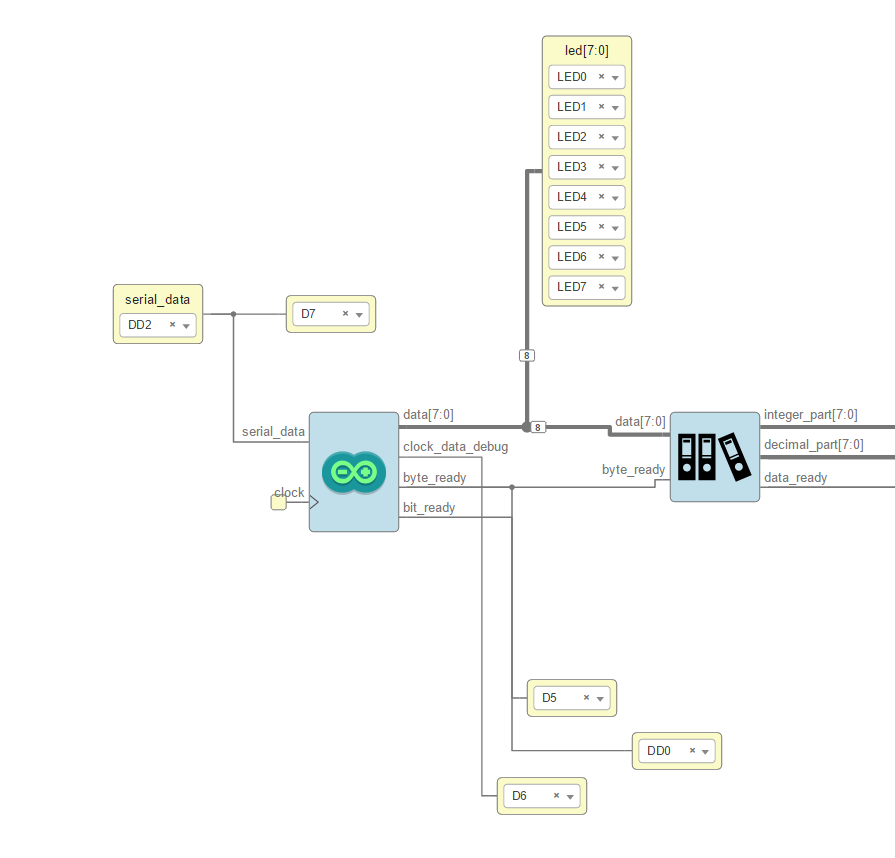
\includegraphics[scale=0.4]{imagenes/Balancing_robot/arduino_arrange.PNG}
	\caption{Communication between Arduino and IceZum Alhambra.}
	\label{fig:arduino_arrange}
\end{figure}


\newpage

\subsection{PID Control in IceZum Alhambra}
As it has been explained in section \ref{sec:PID}, a PID controller can be used in a simple way to control the stability of the system. \newline
One of the facilities in the use of this kinds of controllers is because its ease of implementation.
\subsubsection{Controlador P} \label{sec:ControladorP}
The flow diagram that features the behavior of the P controller is shown in Figure \ref{fig:P_control}.
	\begin{figure}[H]
	\center
	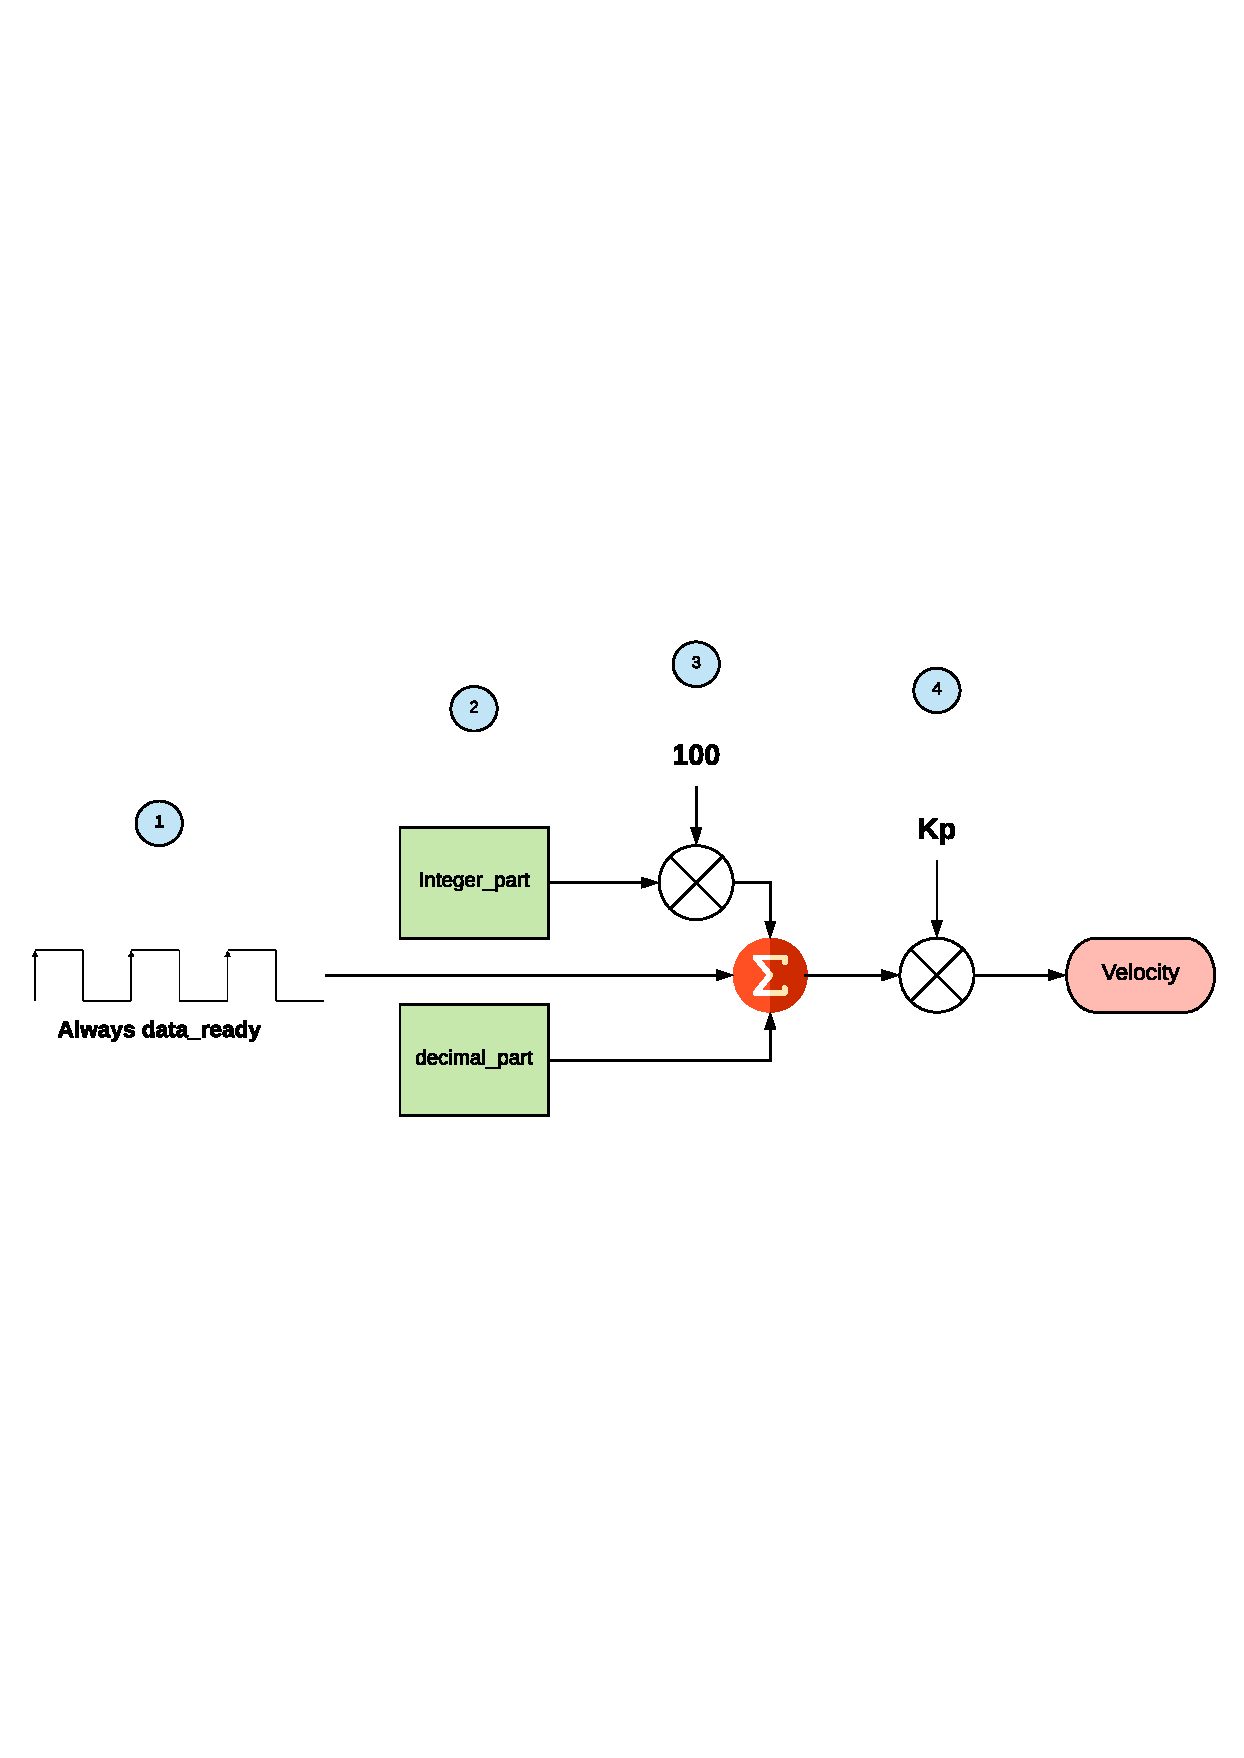
\includegraphics[trim = 0cm 7cm 0mm 7cm, clip,scale=0.5]{imagenes/Balancing_robot/P.pdf}
	\caption{Flow diagram P control.}
	\label{fig:P_control}
\end{figure}

Due to its importance, the functionality is briefly explained ahead:

\begin{itemize}
	\item 1.-The complete process will be refreshed every time there is a new datum, this is in this case, every time the angle system is changing.
	\item 2.-As inputs there are both the integer part as the decimal part from the angle.
	\item 3.-Both the integer part and the decimal part are represented as 8 bits data without sign. So, in order to give more importance to the integer part, there is the option to divide the decimal part by 100 or to multiply the integer part by 100. In the first option there is not a good behavior obtained due to the digital treat of the floating comma, which is why the second option is better.
	\item 4.- At the end, the two integer and decimal components are added and then it is multiplied by a Kp constant, defined as a parameter which can be didactically changed.
\end{itemize}

Its representation in IceStudio has the aspect as shown in Figure \ref{fig:Pcontrol}.

\begin{figure}[H]
	\center
	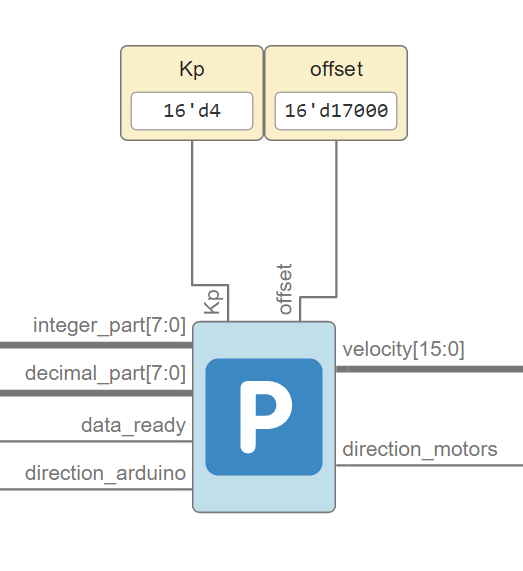
\includegraphics[scale=0.5]{imagenes/Balancing_robot/Pcontrol}
	\caption{Appearance of P control in IceStudio}
	\label{fig:Pcontrol}
\end{figure}
\newpage
\subsubsection{D Controller} \label{sec:ControladorD}

Referring to the D controller, the flow diagram implemented in Verilog is shown in Figure \ref{fig:D_control}. 
	\begin{figure}[H]
	\center
	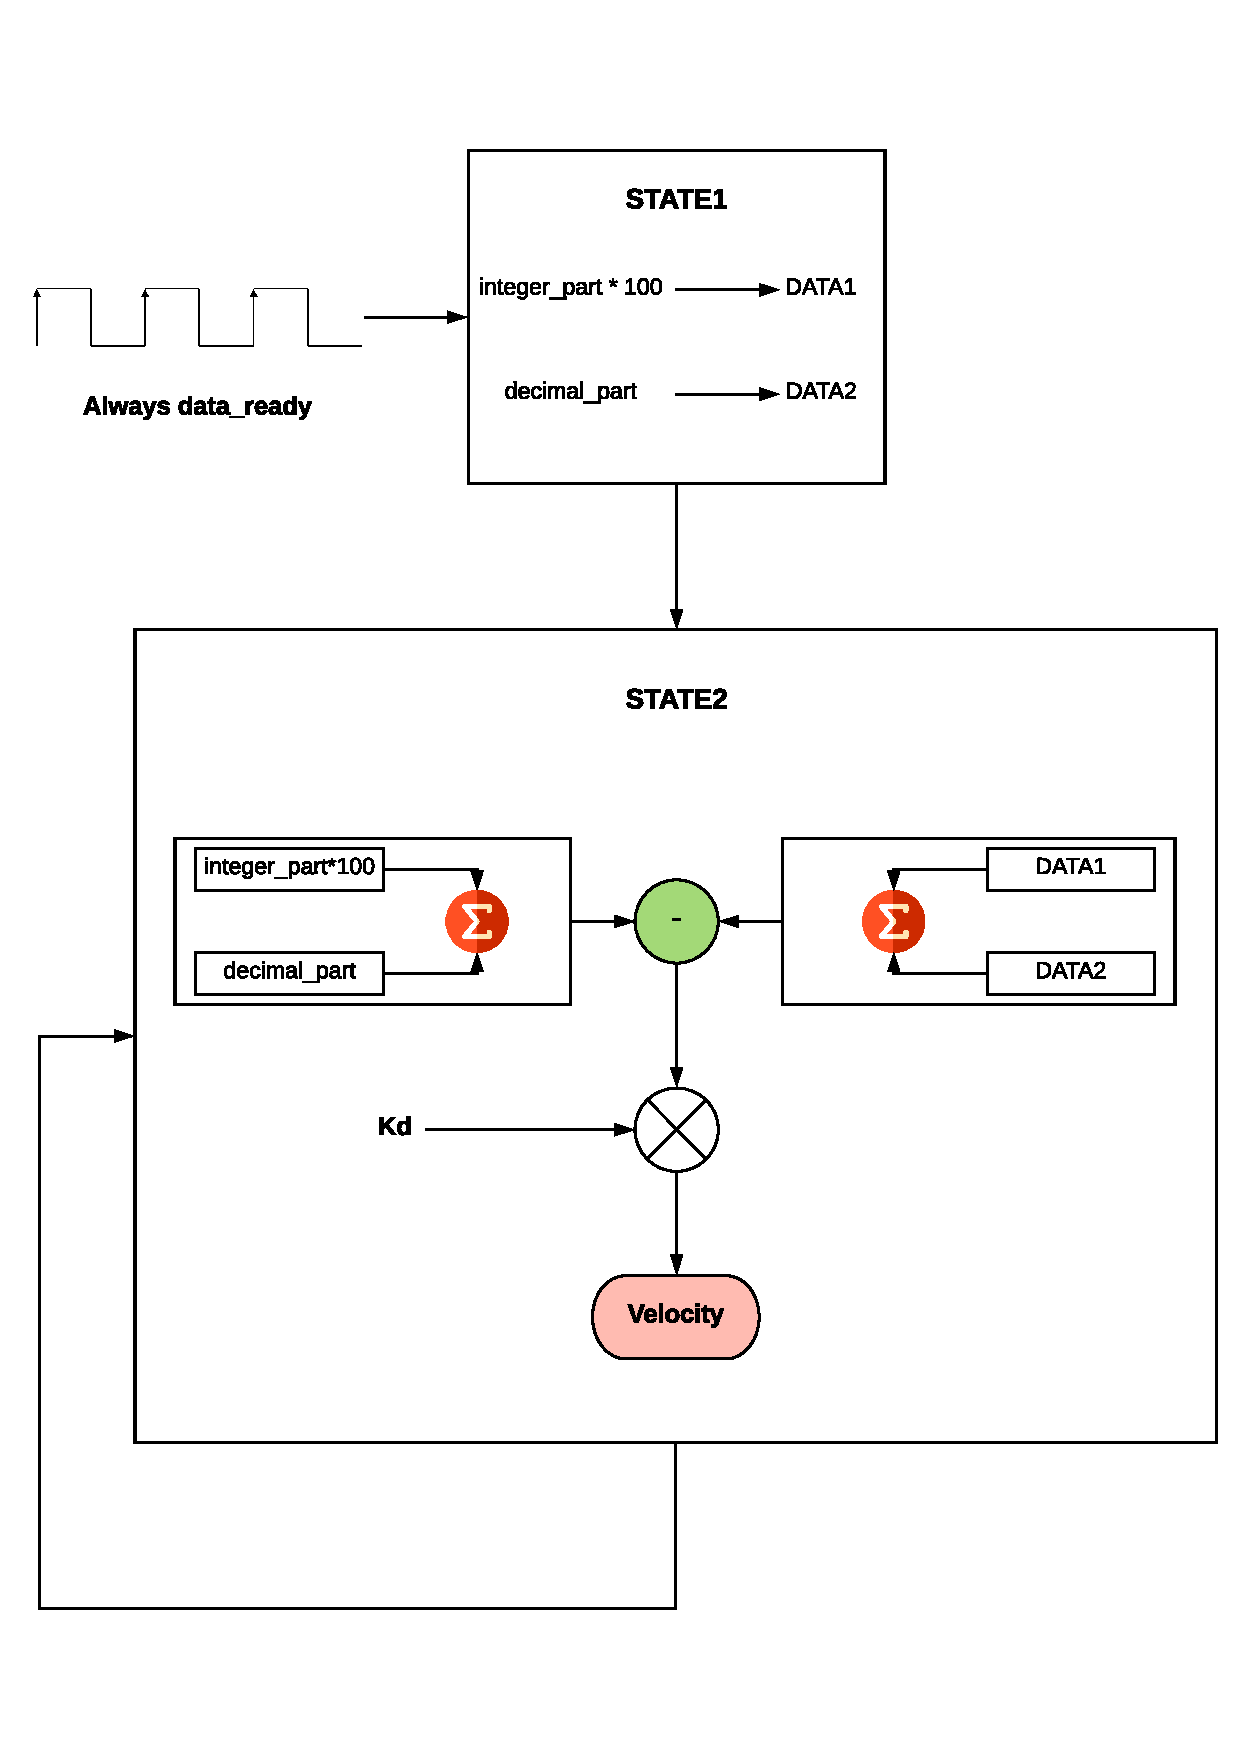
\includegraphics[trim = 0cm 0cm 0mm 0cm, clip,scale=0.4]{imagenes/Balancing_robot/D.pdf}
	\caption{Flow diagram D control.}
	\label{fig:D_control}
\end{figure}

Its implementation is composed by a state machine with two states, which will change at each pulse on the $data_ready$, which means, will change whenever a new angle is available.\newline

If remembered, D controller is based in its operation on the prediction of future errors. The derivative control action generates a control signal proportional to the derivative of the error signal. \newline
A subtraction (derived from the error in time) is therefore carried out between the current error and the last error. Its result is multiplied by the constant Kd. Its representation in IceStudio is represented in \ref{fig:Dcontrol}.

\begin{figure}[H]
	\center
	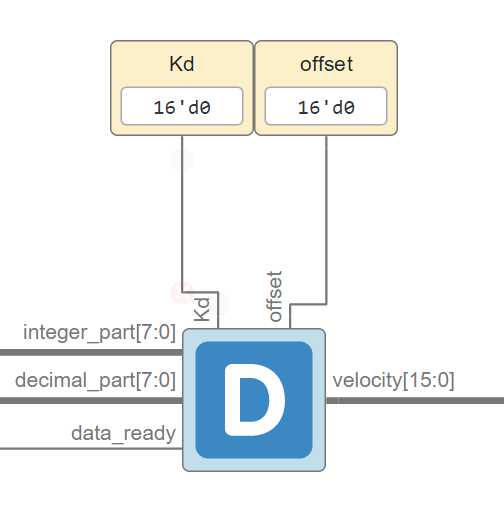
\includegraphics[scale=0.5]{imagenes/Balancing_robot/Dcontrol}
	\caption{Appearance of D control module in IceStudio.}
	\label{fig:Dcontrol}
\end{figure}

\subsubsection{Controlador PD}

Referring to the closed loop feedback system analyzed in section \ref{sec:PID}, it is important to show the final result of the aspect of the present project in IceStudio, making a direct comparison between this (figure \ref{fig:finalIceStudio} ) and figure \ref{fig:PID}.
\newpage
\begin{figure}[H]
	\center
	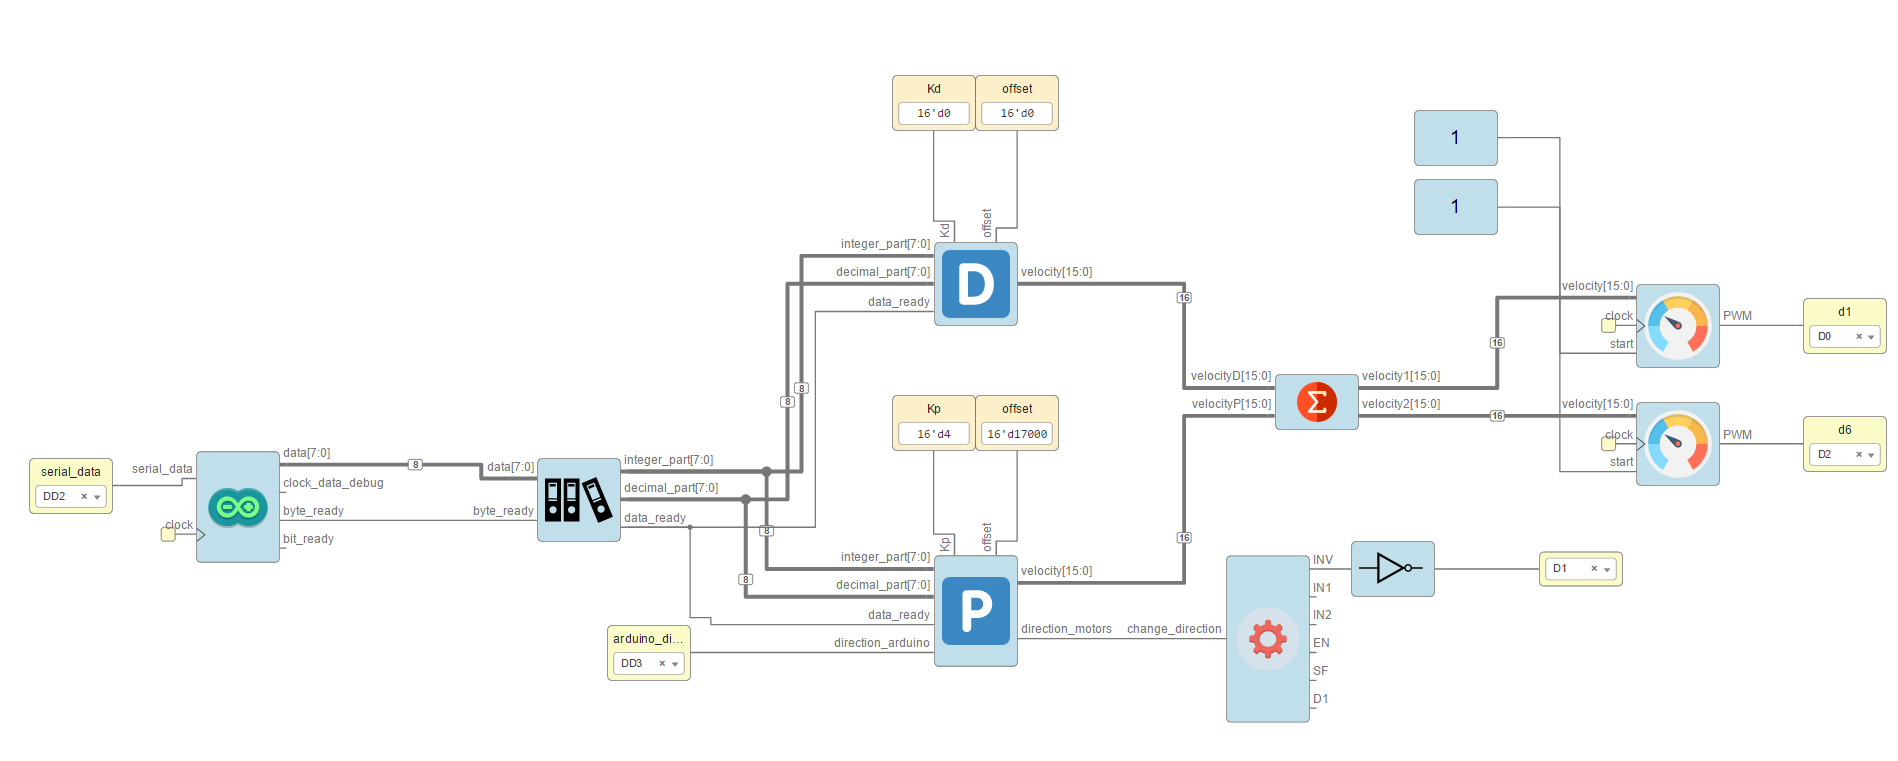
\includegraphics[scale=0.5, angle=90]{imagenes/Balancing_robot/finalIceStudio}
	\caption{Final appearance of Self-Balancin in IceStudio.}
	\label{fig:finalIceStudio}
\end{figure}

\subsection{Motor controller} \label{sec:driver_motores}
Having a module with the ability to generate PWM solves many subsequent problems while improving the visibility of the code in the final system. As can be seen in the motor features, most of them are commanded by a PWM signal that, although it is true, depends on the motor in issue. \newline
Pulse Width Modulation (PWM) is a technique that modifies the work cycle of a periodic signal (squared in our case) that is used to transmit information through a communication channel or to control the amount of energy that is sent to a load. An example of a PWM squared signal is shown in figure \ref{fig:pwm_example}.

\begin{figure}[H]
	\center
	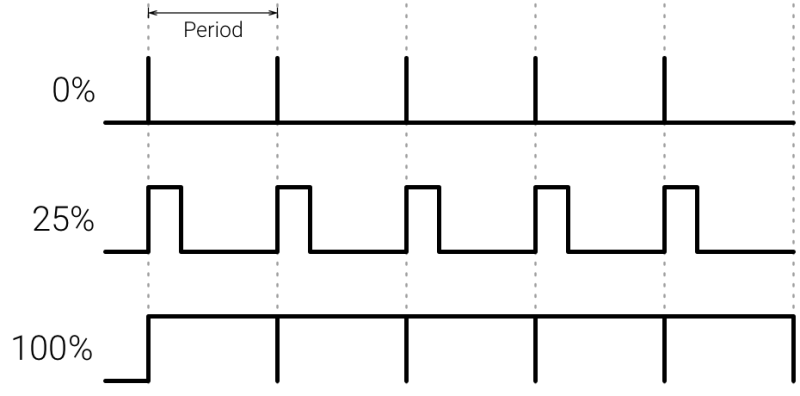
\includegraphics[trim = 0mm 0cm 0mm 0cm, clip,scale=0.4]{imagenes/Balancing_robot/pwm_example.png}
	\caption{PWM signal example with different dutty.}
	\label{fig:pwm_example}
\end{figure}


Applying this signal, for example, to a classic DC motor the amount of energy that is applied to the load is varied, the motor in this case. It simply works as a switch in which a high logical level is open and a low level closed. If it is managed to vary the time the motor is being charged and the time in where there’s no current, you can control its speed. \newline

The features of a PWM signal are: 
\begin{itemize}
	\item D = Work cycle.
	\item $\tau$ = Time-lapse while the function is positive.
	\item T = Function period.
\end{itemize}


The motor driver used to control DC motors (MC33926 [] figure \ref{fig:driver_motor_fisico}),needs a series of configurations to work according to the needs which could be obtained from its datasheet[]. The final inputs and outputs diagram and also the necessary connections are detailed in the scheme of the \ref{fig:driver_motor} figure.


\begin{figure}[H]
	\center
	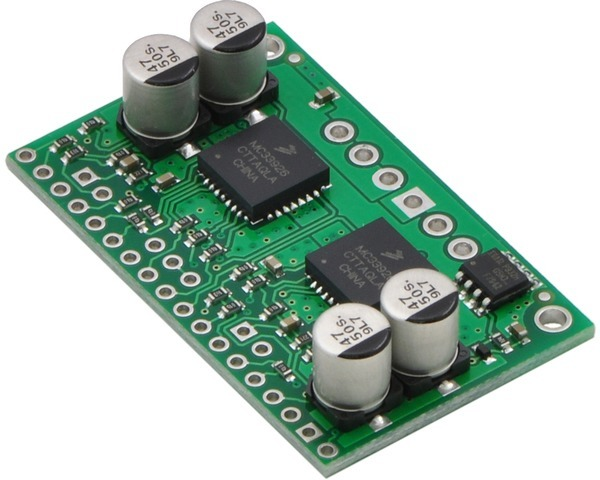
\includegraphics[trim = 0mm 0cm 0mm 0cm, clip,scale=0.4]{imagenes/Balancing_robot/driver_motor.jpg}
	\caption{MC33926 to control DC motors.}
	\label{fig:driver_motor_fisico}
\end{figure}


\begin{figure}[H]
	\center
	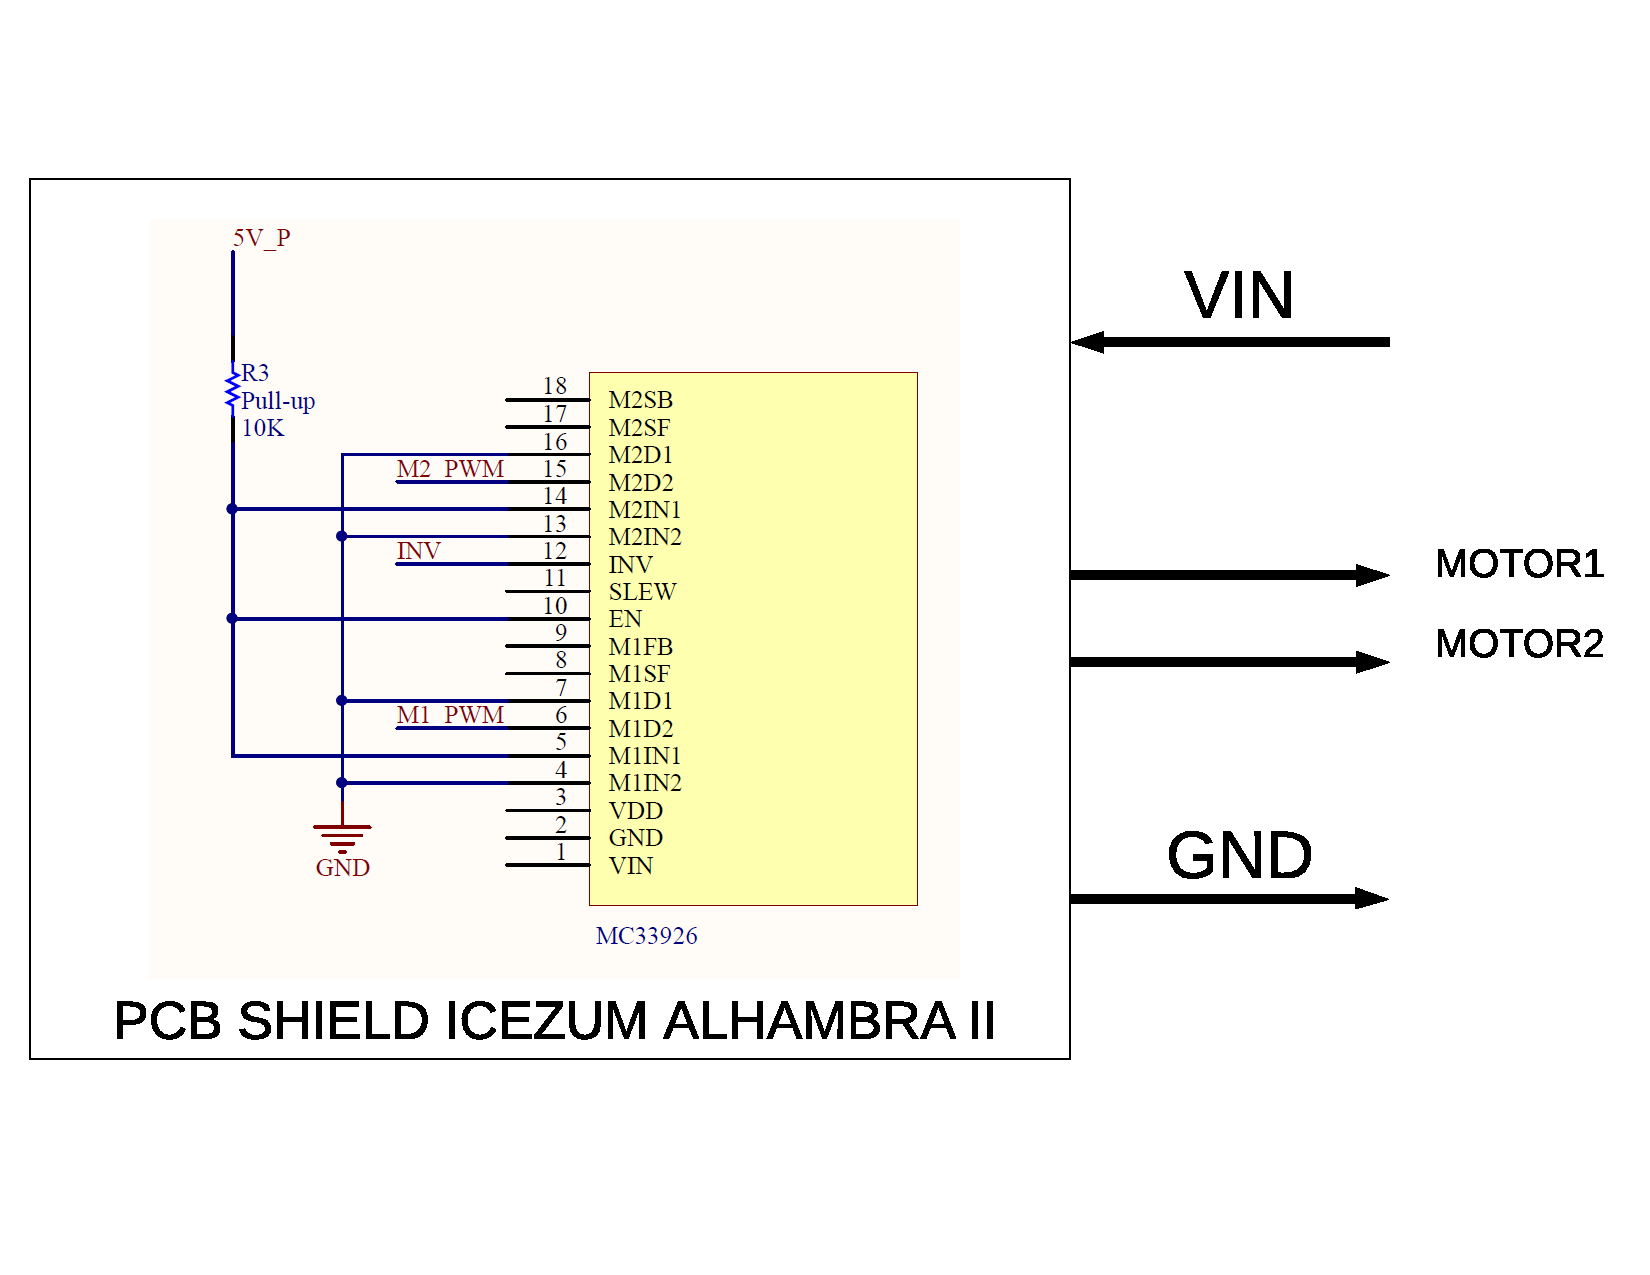
\includegraphics[trim = 0mm 3cm 0mm 2cm, clip,scale=0.4]{imagenes/Balancing_robot/driver_motor.pdf}
	\caption{Schematic MC33926.}
	\label{fig:driver_motor}
\end{figure}




\subsubsection{PWM Control}

The speed of the motors is controlled by a PWM which is connected to pin 15 or M2D2, from figure \ref{fig:driver_motor} for each one of the motors and another PWM generator connected to pin 6 or M1D1 from the DC motor driver. This generator module has the aspect shown in figure \ref{fig:pwm_module} in IceStudio. 

\begin{figure}[H]
	\center
	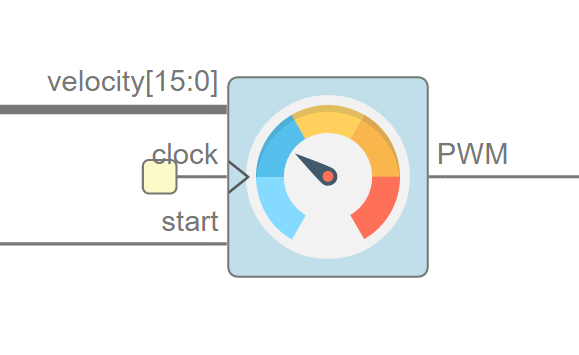
\includegraphics[scale=0.5]{imagenes/Balancing_robot/PWM_module.PNG}
	\caption{Appearance PWM module in IceStudio.}
	\label{fig:pwm_module}
\end{figure}

The block diagram of its performance is exposed in figure \ref{fig:pwm_control}.

\begin{figure}[H]
	\center
	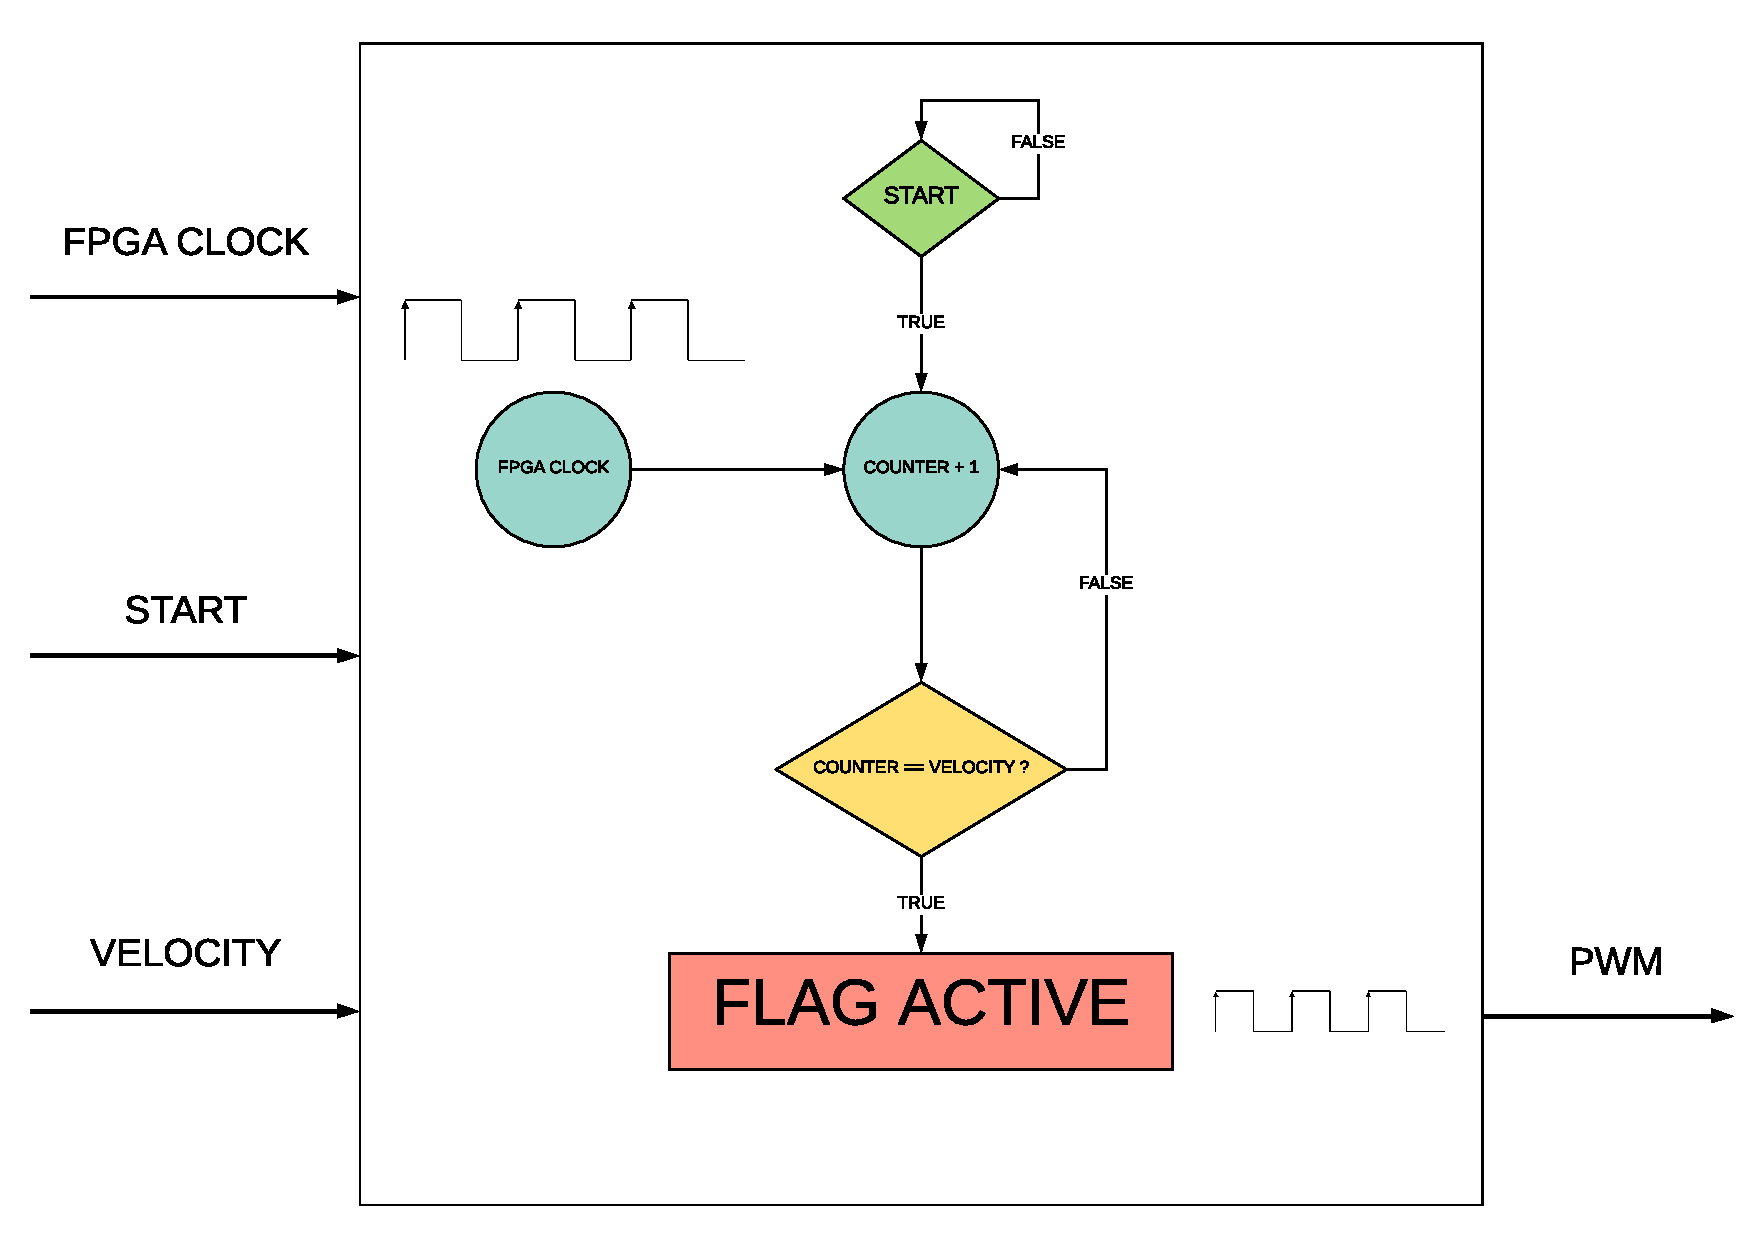
\includegraphics[trim = 0mm 0mm 0mm 0mm, clip,scale=0.4]{imagenes/Balancing_robot/pwm_control.pdf}
	\caption{Flow diagram PWM generator in Verilog.}
	\label{fig:pwm_control}
\end{figure}

Its performance is based in an input clock pulse counter from the FPGA. A speed log will dictate how many pulses have to be counted before an output signal is settled on (desired PWM). As inputs are: \newline 
\begin{itemize}
	\item FPGA Clock: Is the 12Mhz FPGA clock which is in charge of the pulse counter.
	\item Start: It is a common signal to the whole system, performing as a switch to give a general start.
	\item Velocity: Is a record that marks how many clock pulses need to be counted before activating the output signal PWM.
\end{itemize}

As outputs are:
\begin{itemize}
	\item As outputs are:
\end{itemize}



\subsection{Power Supply System}


As with any electronic system, a power source is necessary to allow the correct operation of all the components. \newline

As a fundamental task, an analysis of the requirements of these components that make up the complete system is a priority in order to choose an adequate power supply. In addition, it is considered that the purpose is to have a mobile system and that, as far as possible, a direct connection to the electrical network or a USB connection to a computer is avoided. So, it only remains to choose what type of battery is suitable.\newline

Next, the different types of battery currently in the market are named, analyzing their most important advantages and disadvantages: 

\begin{itemize}
	\item Lead-acid Batteries: They are inexpensive and easy to manufacture but do not admit overloads or deep discharges, besides, they are heavy and have a big volume compared with the small amount of energy they are capable of storing.
	\item Nickel-cadmium Batteries (Ni-Cd): They work well over a wide range of temperatures and can be overloaded without damage. They allow deep discharges and provide a good number of cycles. As in the previous one, they have a very high weight and volume.
	\item Nickel-metal Hydride Batteries (Ni-MH): Features compared to the previous batteries are improved, however, it provides a fewer number of cycles.
	\item Lithium Ion Batteries (Li-ion): In comparison with the previous ones, these are from a recent development and have facilitated the existence of portable technologies. They have a high capacity in relation to their weight and volume, they have a very high self-discharge factor. They are almost unaffected by the
	memory effect and can be charged without having been previously discharged. On the other hand, they do not support temperature changes too good.
	\item Lithium Polymer Batteries (Li-Po): They are a variation of the Li-ion batteries that improve their weight and volume features as its discharge rate. They remain practically unused if they are discharged in excess.
\end{itemize}

Considering that the final and most restrictive system is a remotely piloted aerial vehicle, and that the self-balance robot needs a not very high weight, it is important that the weight features, volume, and discharge are adequate. For this reason, Li-po type batteries are chosen for the power supply of the systems in this project, which can store a large amount of energy and offer a very high discharge rate. \newline

The Li-Po type batteries have a different nomenclature from the rest, which is necessary to analyze:

\begin{itemize}
	\item Sort by number of cells "S": The number S corresponds to the number of cells, which are 3.7 volts but can reach 4.2 if they are fully charged. A 3-cell (3S) battery is composed of 3 sub-batteries placed in series, which is, a total of 11.1 volts.
	\item Capacity indicated in "mAh”: The higher the number of mAh, the higher the load capacity. A common mistake is to think that the greater the capacity, the greater the possibility of lengthening the time of the system in issue. At higher capacity, weight and volume of the battery increase, so the best configuration for this system must be found.
	\item TDownload rate "C": The number from C corresponds to the battery discharge rate. If a battery is 1C, it means that the maximum discharge rate it can reach is the one corresponding to its capacity. If the number C is different from 1 means that we multiply the discharge rate by that value, reducing the discharge time proportionally, that is, a battery of 1000mAh 2C will be discharged to 2A in half an hour.
\end{itemize}

The following approach will be to choose which of the previous values is the most adequate for the system. For this and after analyzig the differents components separately, two independent subsystems are distinguished in terms of the power supply:

\begin{itemize}
	\item DC Motors and Arduino Nano Power Supply.
	\item IceZum Alhambra II and other components Power Supply.
\end{itemize}

\subsubsection{DC Motors and Arduino Nano Power Supply}
For the DC motors and Arduino Nano power supply, a 11.1V and 2200mAh LIPO battery of is used as in figure \ref{fig:lipo111}. As it is presented in the final schematic from the controller
shield (Figure \ref{fig:schematics_tfg}), the battery is connected to the shield, which is in charge to supply both the motors and Arduino Nano.

\begin{center}
	\begin{figure}[H]
		\center
		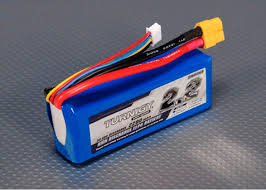
\includegraphics[scale=0.8]{imagenes/Balancing_Robot/LIPO111}
		\caption{LIPO Battery 11.1V y 2.2A. }
		\label{fig:lipo111}
	\end{figure}
\end{center}

\subsubsection{Alhambra IceZum II and other components Power Supply}

For the IceZum Alhambra II power supply and the rest of the components, a 3.7V and 4mAh LIPO battery has been used, as shown in Figure \ref{fig:lipo37}. 
\begin{center}
	\begin{figure}[H]
		\center
		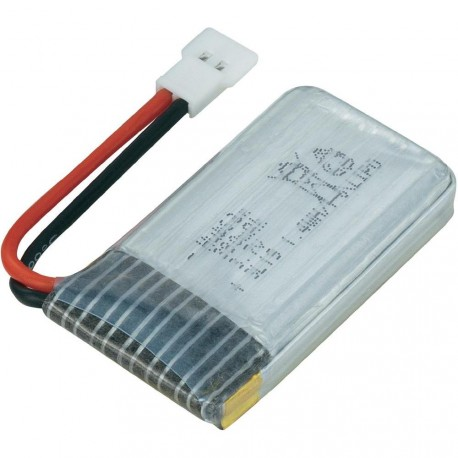
\includegraphics[scale=0.5]{imagenes/Balancing_Robot/LIPO37}
		\caption{LIPO Battery 3.7V y 4mAh.}
		\label{fig:lipo37}
	\end{figure}
\end{center}
\newpage
\subsection{Materials and Prototype Cost}
In the table \ref{tabla:coste} the total cost of the prototype along chapter \ref{sec: BalancingRobot} is pulled apart.
It is differenciated by four columns called material, number of units, unit cost and total cost in euros.
\begin{table}[H]
	\scalebox{0.9}{
	\begin{turn}{90}
	\begin{tabular}{|l|l|l|l|l}
		\cline{1-4}
		\multicolumn{1}{|c|}{\cellcolor[HTML]{FFCE93}\textbf{MATERIAL}} & \cellcolor[HTML]{FFCE93}\textbf{QUANTITY} & \multicolumn{1}{c|}{\cellcolor[HTML]{FFCE93}\textbf{\begin{tabular}[c]{@{}c@{}}UNIT \\ COST (\euro)\end{tabular}}} & \multicolumn{1}{c|}{\cellcolor[HTML]{FFCE93}\textbf{\begin{tabular}[c]{@{}c@{}}TOTAL \\ COST (\euro)\end{tabular}}} &  \\ \cline{1-4}
		IceZum Alhambra II                                               & 1                                         & 60                                                                                                                  & 60                                                                                                               &  \\ \cline{1-4}
		Arduino Nano                                                    & 1                                         & 8                                                                                                                   & 8                                                                                                                &  \\ \cline{1-4}
		Hexagonal Nylon 10 mm Separator                                 & 4                                         & 0.20                                                                                                                & 0.80                                                                                                             &  \\ \cline{1-4}
		Metálico Hexagonal M3 25 mm Separator                           & 8                                         & 0.25                                                                                                                & 2                                                                                                                &  \\ \cline{1-4}
		Metálico Hexagonal M3 50 mm Separator                           & 4                                         & 0.41                                                                                                                & 1.64                                                                                                             &  \\ \cline{1-4}
		Nylon M3 Screw                                               & 16                                        & 0.09                                                                                                                & 1.44                                                                                                             &  \\ \cline{1-4}
		Nylon M3 Nut                                                 & 8                                         & 0.05                                                                                                                & 0.40                                                                                                             &  \\ \cline{1-4}
		Nylon M1 Screw                                               & 4                                         & 0.09                                                                                                                & 0.39                                                                                                             &  \\ \cline{1-4}
		Nylon M1 Nut                                                 & 8                                         & 0.05                                                                                                                & 0.40                                                                                                             &  \\ \cline{1-4}
		PCB 4 layers                               & 1                                         & 5                                                                                                                   & 5                                                                                                                &  \\ \cline{1-4}
		Wheel 7 cm                                                      & 2                                         & 7.90                                                                                                                & 15.80                                                                                                            &  \\ \cline{1-4}
		Motor DC                                                        & 2                                         & 24.95                                                                                                               & 49.9                                                                                                             &  \\ \cline{1-4}
		Driver Motor DC Dual MC33926                                    & 1                                         & 30                                                                                                                  & 30                                                                                                               &  \\ \cline{1-4}
		IMU MPU6050                                                     & 1                                         & 2.50                                                                                                                & 2.50                                                                                                             &  \\ \cline{1-4}
		Mechanical 3D Structure                                         & 1                                         & 20                                                                                                                  & 20                                                                                                               &  \\ \cline{1-4}
		Screw 3.5 mm                                                    & 5                                         & 0.80                                                                                                                & 4                                                                                                                &  \\ \cline{1-4}
		Cable 5-pin                                                     & 1                                         & 0.82                                                                                                                & 0.82                                                                                                             &  \\ \cline{1-4}
		PIN 2,54 mm 4 contacts Macho                           & 1                                         & 0.08                                                                                                                & 0.08                                                                                                             &  \\ \cline{1-4}
		PIN 2,54 mm 8 contacts Shield                          & 2                                         & 0.54                                                                                                                & 1.08                                                                                                             &  \\ \cline{1-4}
		PIN 2,54 mm 6 contacts Shield                          & 2                                         & 0.58                                                                                                                & 1.16                                                                                                             &  \\ \cline{1-4}
		Jumper 2.54 mm                               & 2                                         & 0.08                                                                                                                & 0.16                                                                                                             &  \\ \cline{1-4}
		PIN 2,54 mm 10 contacts Female                         & 2                                         & 0.10                                                                                                                & 0.20                                                                                                             &  \\ \cline{1-4}
		PIN 2,54 mm 10 contacts Male                          & 5                                         & 0.10                                                                                                                & 0.50                                                                                                             &  \\ \cline{1-4}
		Resistance 4K7 5\%                                             & 3                                         & 0.21                                                                                                                & 0.63                                                                                                             &  \\ \cline{1-4}
		Tin                                                          & 1                                         & 5.50                                                                                                                & 5.50                                                                                                             &  \\ \cline{1-4}
		Retractable therman Tape                                    & 2                                         & 1.50                                                                                                                & 3                                                                                                                &  \\ \cline{1-4}
		Cable 12 AWG                                           & 1                                         & 0.90                                                                                                                & 0.90                                                                                                             &  \\ \cline{1-4}
		Battery Lipo 11.1 V 2200 mA                                     & 1                                         & 19.95                                                                                                               & 19.95                                                                                                            &  \\ \cline{1-4}
		Battery Lipo 3.7 V 5 mA                                         & 1                                         & 4.20                                                                                                                & 4.20                                                                                                             &  \\ \cline{1-4}
		\multicolumn{2}{|c|}{}                                                                                      & \multicolumn{2}{c|}{\cellcolor[HTML]{FD6864}}                                                                                                                                                                                          &  \\
		\multicolumn{2}{|c|}{\multirow{-2}{*}{\textbf{PROTOTYPE TOTAL COST:}}}                                     & \multicolumn{2}{c|}{\multirow{-2}{*}{\cellcolor[HTML]{FD6864}\textbf{240.45 \euro}}}                                                                                                                                                         &  \\ \cline{1-4}
	\end{tabular}
	\end{turn}}
	\caption{Total cost of Self-Balancing Robot.}
	\label{tabla:coste}
\end{table}
\newpage
\section{Experiments and final results}
\subsection{Self-Balancing Robot}
\newline 
A set of demostrative video of the correct behaviour in the Self-Balancing robot can be seen in \cite{self2}. Also, the process to the end in \cite{self1} \cite{self3}.\newline

In order to manufacture the mechanical structure, a 3D printer was used \cite{print1}.

A set of images wich form the final system are shown in \ref{fig:test1}, \ref{fig:test2}.

\begin{center}
\begin{figure}[H]
	\center
	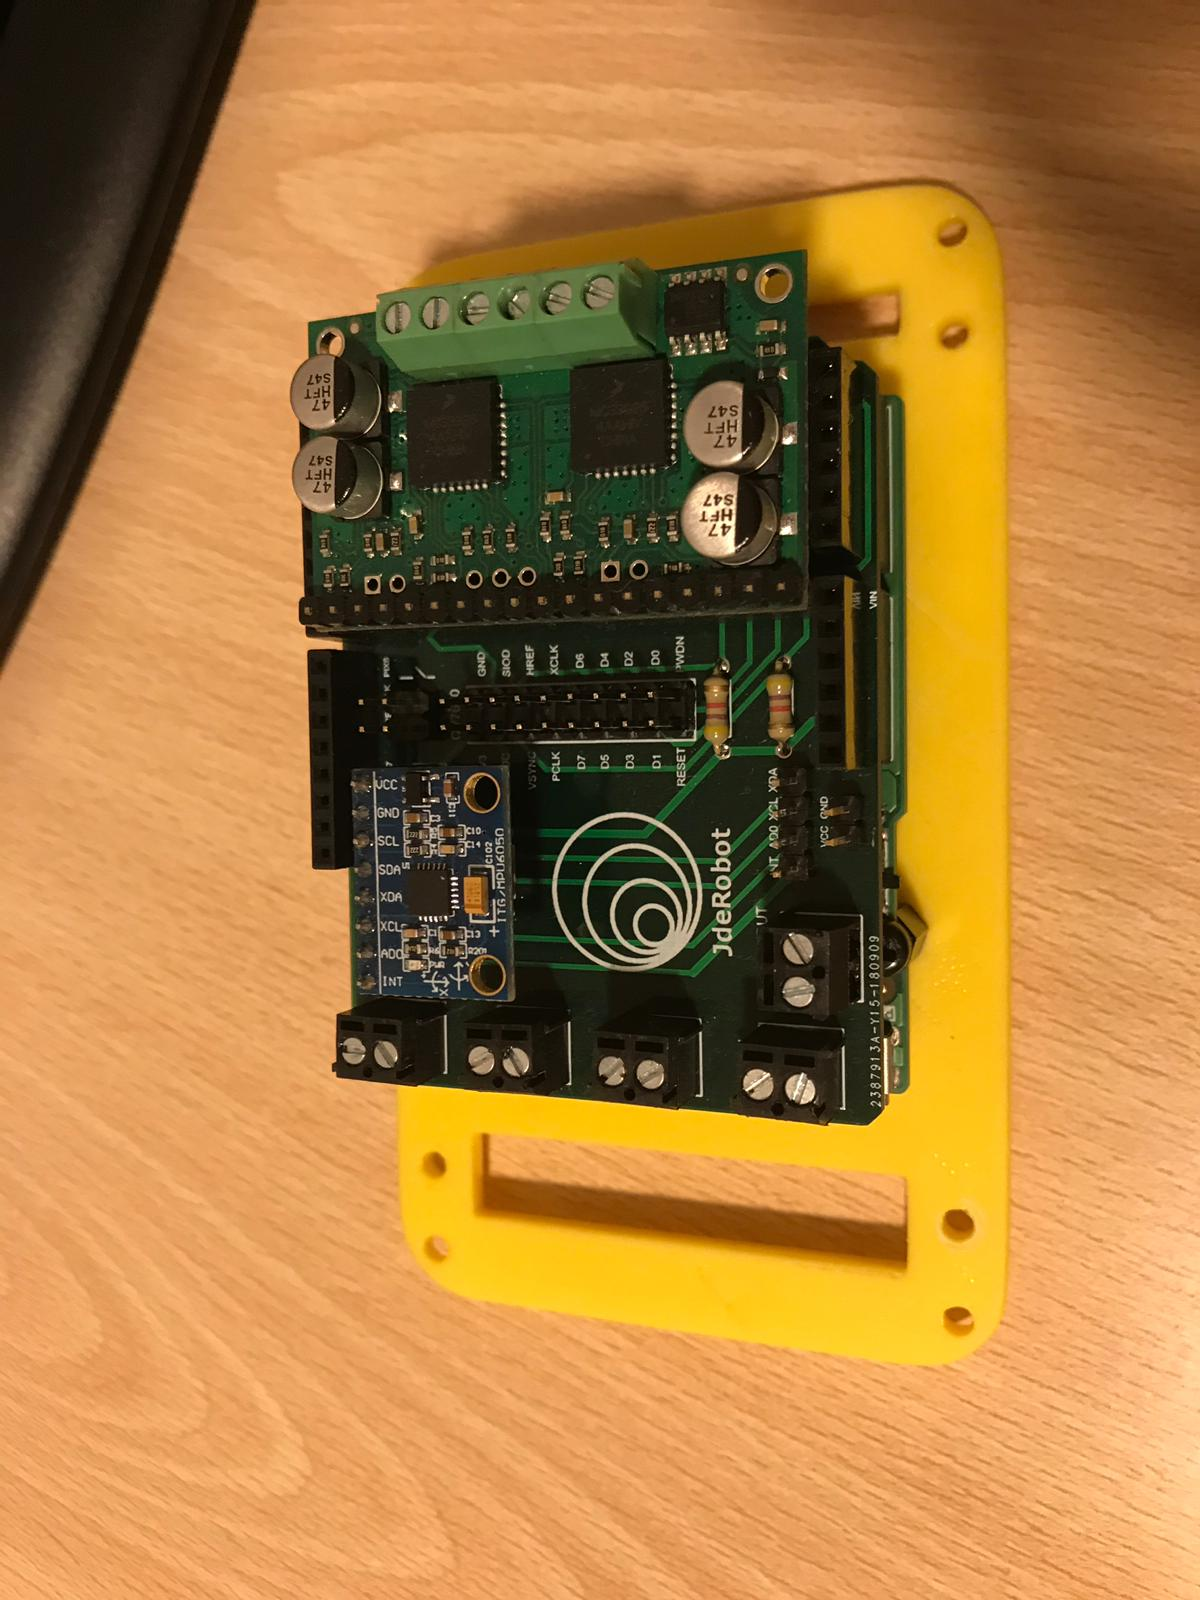
\includegraphics[scale=0.2, angle=270]{imagenes/Balancing_Robot/test1}
	\caption{}
	\label{fig:test1}
\end{figure}
\end{center}

\begin{center}
	\begin{figure}[H]
		\center
		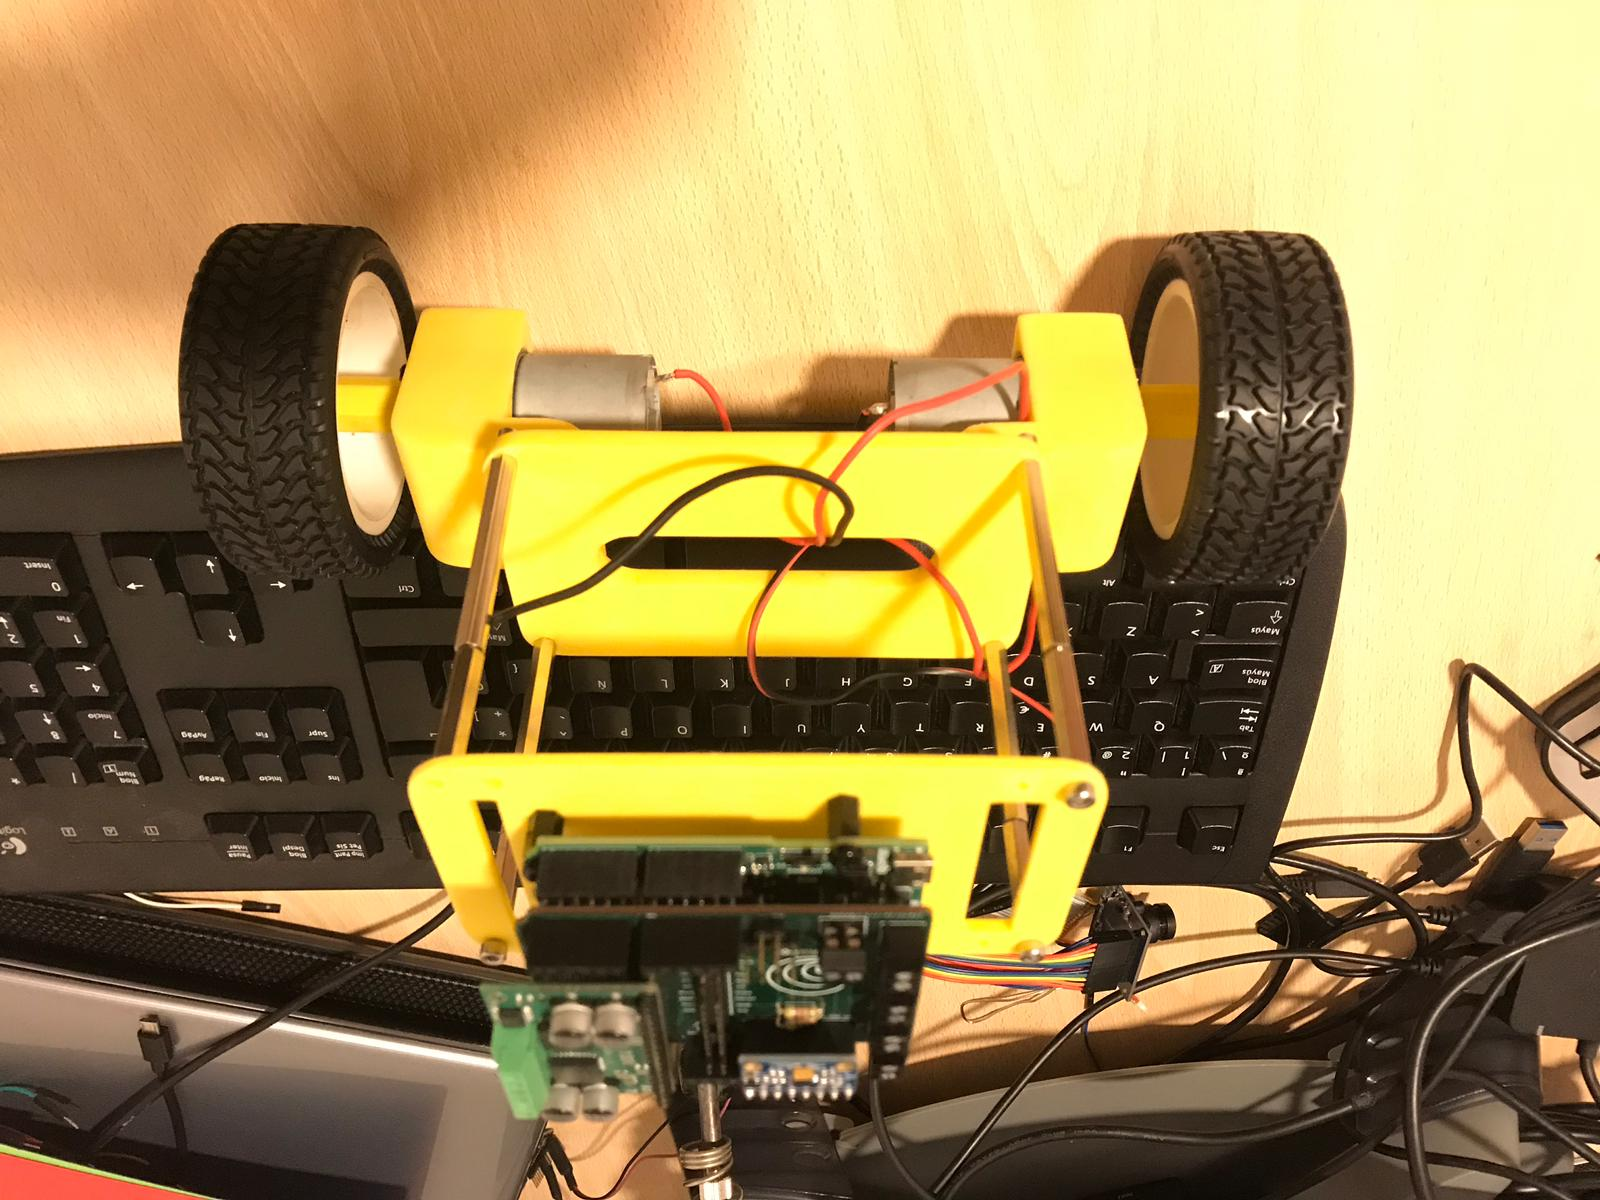
\includegraphics[scale=0.2, angle=180]{imagenes/Balancing_Robot/test2}
		\caption{}
		\label{fig:test2}
	\end{figure}
\end{center}

\subsection{VGA Module}
For a more adequate knowledge of the hardware implementation language Verilog, prior to the realization of this project and as an initial idea to use it in future projects, a shield is carried out for the connection with a screen, having to know for it this communication protocol. A video demonstration is found in \cite{vga}. \newline
The manufactured shield is represented in the figure \ref{fig:vga}

\begin{center}
	\begin{figure}[H]
		\center
		\includegraphics[scale=0.2]{imagenes/Balancing_Robot/vga}
		\caption{}
		\label{fig:vga}
	\end{figure}
\end{center}
\subsection{Motor brushless Controller}
With the fundamental idea of using the PCB for a totally independent quad-copter system and as a first approximation to the control of brushless motors, the model of the figure is developed such that it allows a control over this type of actuators.
A demonstration video can be found in \cite{brushless1}.